% ------------------------------------------------------------
% LaTeX Template für die DHBW zum Schnellstart!
% Original: https://github.wdf.sap.corp/vtgermany/LaTeX-Template-DHBW
% ------------------------------------------------------------
% ---- Präambel mit Angaben zum Dokument
\documentclass[
	fontsize=12pt,           % Leitlinien sprechen von Schriftgröße 12.
	paper=A4,
	twoside=false,
	listof=totoc,            % Tabellen- und Abbildungsverzeichnis ins Inhaltsverzeichnis
	bibliography=totoc,      % Literaturverzeichnis ins Inhaltsverzeichnis aufnehmen
	titlepage,               % Titlepage-Umgebung anstatt \maketitle
	headsepline,             % horizontale Linie unter Kolumnentitel
	abstract,              % Überschrift einschalten, Abstract muss in {abstract}-Umgebung stehen
]{scrreprt}                  % Verwendung von KOMA-Report
\usepackage[utf8]{inputenc}  % UTF8 Encoding einschalten
\usepackage[english]{babel}  % Neue deutsche Rechtschreibung
\usepackage[T1]{fontenc}     % Ausgabe von westeuropäischen Zeichen (auch Umlaute)
\usepackage{microtype}       % Trennung von Wörtern wird besser umgesetzt
\usepackage{lmodern}         % Nicht-gerasterte Schriftarten (bei MikTeX erforderlich)
\usepackage{graphicx}        % Einbinden von Grafiken erlauben
\usepackage{wrapfig}         % Grafiken fließend im Text
\usepackage{setspace}        % Zeilenabstand \singlespacing, \onehalfspaceing, 
\doublespacing
\usepackage[
	%showframe,                % Ränder anzeigen lassen
	left=2.7cm, right=2.5cm,
	top=2.5cm,  bottom=2.5cm,
	includeheadfoot
]{geometry}                      % Seitenlayout einstellen
\usepackage{scrlayer-scrpage}    % Gestaltung von Fuß- und Kopfzeilen
\usepackage{acronym}             % Abkürzungen, Abkürzungsverzeichnis
\usepackage{titletoc}            % Anpassungen am Inhaltsverzeichnis
\contentsmargin{0.75cm}          % Abstand im Inhaltsverzeichnis zw. Punkt und Seitenzahl
\usepackage[                     % Klickbare Links (enth. auch "nameref", "url" Package)
  hidelinks,                     % Blende die "URL Boxen" aus.
  breaklinks=true                % Breche zu lange URLs am Zeilenende um
]{hyperref}
\usepackage[hypcap=true]{caption}% Anker Anpassung für Referenzen
\urlstyle{same}                  % Aktuelle Schrift auch für URLs
% Anpassung von autoref für Gleichungen (ergänzt runde Klammern) und Algorithm.
% Anstatt "Listing" kann auch z.B. "Code-Ausschnitt" verwendet werden. Dies sollte
% jedoch synchron gehalten werden mit \lstlistingname (siehe weiter unten).
%\addto\extrasngerman{%
%	\def\equationautorefname~#1\null{Gleichung~(#1)\null}
%	\def\lstnumberautorefname{Zeile}
%	\def\lstlistingautorefname{Listing}
%	\def\algorithmautorefname{Algorithmus}
	% Damit einheitlich "Abschnitt 1.2[.3]" verwendet wird und nicht "Unterabschnitt 1.2.3"
	% \def\subsectionautorefname{Abschnitt}
%}

% ---- Abstand verkleinern von der Überschrift 
\renewcommand*{\chapterheadstartvskip}{\vspace*{.5\baselineskip}}

% Hierdurch werden Schusterjungen und Hurenkinder vermieden, d.h. einzelne Wörter
% auf der nächsten Seite oder in einer einzigen Zeile.
% LaTeX kann diese dennoch erzeugen, falls das Layout ansonsten nicht umsetzbar ist.
% Diese Werte sind aber gute Startwerte.
\widowpenalty10000
\clubpenalty10000

% ---- Für das Quellenverzeichnis
\usepackage[
	backend = biber,                % Verweis auf biber
	language = auto,
	style = numeric,                % Nummerierung der Quellen mit Zahlen
	sorting = nty,                 % none = Sortierung nach der Erscheinung im Dokument
	sortcites = true,               % Sortiert die Quellen innerhalb eines cite-Befehls
	block = space,                  % Extra Leerzeichen zwischen Blocks
	hyperref = true,                % Links sind klickbar auch in der Quelle
	%backref = true,                % Referenz, auf den Text an die zitierte Stelle
	bibencoding = auto,
	giveninits = true,              % Vornamen werden abgekürzt
	%doi=false,                      % DOI nicht anzeigen
	isbn=false,                     % ISBN nicht anzeigen
    alldates=iso,                  % Datum immer als DD.MM.YYYY anzeigen
	%url=false
]{biblatex}
\DeclareFieldFormat[article]{volume}{Vol. #1}
\DeclareFieldFormat[article]{number}{, No. #1}
\renewbibmacro*{journal+issuetitle}{%
	\usebibmacro{journal}%
	\setunit*{\addcomma\space}%
	\iffieldundef{series}
	{}
	{\newunit
	\printfield{series}%
	\setunit{\addspace}}%
	\usebibmacro{volume+number+eid}%
	\setunit{\addspace}%
	\usebibmacro{issue+date}%
	\setunit{\addcolon\space}%
	\usebibmacro{issue}%
	\newunit}
\renewbibmacro*{doi+eprint+url}{%
    \printfield{doi}%
    \newunit\newblock%
    \iftoggle{bbx:eprint}{%
        \usebibmacro{eprint}%
    }{}%
    \newunit\newblock%
    \iffieldundef{doi}{%
        \usebibmacro{url+urldate}}%
    {}%
}
\addbibresource{Inhalt/literatur.bib}
\setcounter{biburlnumpenalty}{3000}     % Umbruchgrenze für Zahlen
\setcounter{biburlucpenalty}{6000}      % Umbruchgrenze für Großbuchstaben
\setcounter{biburllcpenalty}{9000}      % Umbruchgrenze für Kleinbuchstaben
\DeclareNameAlias{default}{family-given}  % Nachname vor dem Vornamen
\AtBeginBibliography{\renewcommand{\multinamedelim}{\addslash\space
}\renewcommand{\finalnamedelim}{\multinamedelim}}  % Schrägstrich zwischen den Autorennamen
\DefineBibliographyStrings{german}{
  urlseen = {Last visited },                      % Ändern des Titels von "besucht am"
}
\usepackage[babel,german=quotes]{csquotes}         % Deutsche Anführungszeichen + Zitate

% ---- Für Mathevorlage
\usepackage{amsmath}    % Erweiterung vom Mathe-Satz
\usepackage{amssymb}    % Lädt amsfonts und weitere Symbole
\usepackage{MnSymbol}   % Für Symbole, die in amssymb nicht enthalten sind.


% ---- Für Quellcodevorlage
\usepackage{scrhack}                    % Hack zur Verw. von listings in KOMA-Script
\usepackage{listings}                   % Darstellung von Quellcode
\usepackage{xcolor}                     % Einfache Verwendung von Farben
\input{Inhalt/00_Latex/quellcodeStyle}  % Weitere Details sind ausgelagert

\usepackage{algorithm}                  % Für Algorithmen-Umgebung (ähnlich wie lstlistings Umgebung)
\usepackage{algpseudocode}              % Für Pseudocode. Füge "[noend]" hinzu, wenn du kein "endif",
                                        % etc. haben willst.

\makeatletter                           % Sorgt dafür, dass man @ in Namen verwenden kann.
                                        % Ansonsten gibt es in der nächsten Zeile einen Compilefehler.
\renewcommand{\ALG@name}{Algorithmus}   % Umbenennen von "Algorithm" im Header der Listings.
\makeatother                            % Zeichen wieder zurücksetzen
\renewcommand{\lstlistingname}{Listing} % Erlaubt das Umbenennen von "Listing" in anderen Titel.

% ---- Tabellen
\usepackage{booktabs}  % Für schönere Tabellen. Enthält neue Befehle wie \midrule
\usepackage{multirow}  % Mehrzeilige Tabellen
\usepackage{siunitx}   % Für SI Einheiten und das Ausrichten Nachkommastellen
\sisetup{locale=DE, range-phrase={~bis~}, output-decimal-marker={,}} % Damit ein Komma und kein Punkt verwendet wird.
\usepackage{xfrac} % Für siunitx Option "fraction-function=\sfrac"

% ---- Für Definitionsboxen in der Einleitung
\usepackage{amsthm}                     % Liefert die Grundlagen für Theoreme
\usepackage[framemethod=tikz]{mdframed} % Boxen für die Umrandung
\input{Inhalt/00_Latex/highlightBoxen}  % Weitere Details sind ausgelagert

% ---- Für Todo Notes
\usepackage{todonotes}
\setlength {\marginparwidth }{2cm}      % Abstand für Todo Notizen
\usepackage{multicol}
\usepackage{enumitem}
\setenumerate{nolistsep}
\setitemize{nolistsep}
\DeclareFieldFormat{postnote}{#1}
\DeclareFieldFormat{multipostnote}{#1}

% ---- Elektronische Version oder Gedruckte Version?
% ---- Unterschied: Die elektronische Version enthält keinen Platzhalter für die Unterschrift
\usepackage{ifthen}
\newboolean{e-Abgabe}
\setboolean{e-Abgabe}{false}    % false=gedruckte Fassung

% ---- Persönlichen Daten:
\newcommand{\titel}{Enhancing insights into spending through aggregation with automated document clustering of a large-scale multilingual corpus}
\newcommand{\titelheader}{ }
\newcommand{\arbeit}{Bachelor Thesis}
\newcommand{\studiengang}{Internationale Wirtschaftsinformatik}
\newcommand{\studienjahr}{2019}
\newcommand{\autor}{Lisa Schmidt}
\newcommand{\autorReverse}{Schmidt, Lisa}
\newcommand{\verfassungsort}{Ludwigshafen}
\newcommand{\matrikelnr}{631971}
\newcommand{\kurs}{IBAIT19}
\newcommand{\bearbeitungsmonat}{Januar 2018}
\newcommand{\abgabe}{07.06.2022}
\newcommand{\bearbeitungszeitraum}{01.10.2017 - 31.01.2018}
\newcommand{\firmaName}{SAP SE}
\newcommand{\firmaStrasse}{Dietmar-Hopp-Allee 16}
\newcommand{\firmaPlz}{69190 Walldorf, Deutschland}
\newcommand{\betreuerFirma}{Dr. Karthik Muthuswamy}
\newcommand{\betreuerDhbw}{Prof. Dr. Joachim Melcher}

\input{Inhalt/00_Latex/kopfundFusszeile}

% ---- Hilfreiches
\newcommand{\zB}{z.\,B. }   % "z.B." mit kleinem Leeraum dazwischen (ohne wäre nicht korrekt)
\newcommand{\dash}{d.\,h. }

\newcommand{\code}[1]{\texttt{#1}} % Ist einfacher zu schreiben als ständig \texttt und erlaubt
                                   % Änderungen im Nachhinein, wenn man z.B. Inline-Code anders stylen möchte.

% ---- Silbentrennung (falls LaTeX defaults falsch / nicht gewünscht sind)
\hyphenation{HANA}         % anstatt HA-NA
\hyphenation{Graph-Script} % anstatt GraphS-cript

% ---- Beginn des Dokuments
\begin{document}
\setlength{\parindent}{0pt}              % Keine Paragraphen Einrückung.
                                         % Dafür haben wir den Abstand zwischen den Paragraphen.
\setcounter{secnumdepth}{2}              % Nummerierungstiefe fürs Inhaltsverzeichnis
                 % Tiefe des Inhaltsverzeichnisses. Ggf. so anpassen,
                                         % dass das Verzeichnis auf eine Seite passt.
\sffamily                                % Serifenlose Schrift verwenden.

% ---- Vorspann
% ------ Titelseite
\singlespacing
\thispagestyle{empty}
\begin{titlepage}
\enlargethispage{4cm}

\begin{figure}           % Logo vom Ausbildungsbetrieb und der DHBW
	\vspace*{-5mm} % Sollte dein Titel zu lang werden, kannst du mit diesem "Hack" 
	%                  den Inhalt der Seite nach oben schieben.
	\begin{minipage}{0.49\textwidth}
		\flushleft
		\includegraphics[height=2.5cm]{Bilder/Logos/Logo_SAP.pdf} 
	\end{minipage}
	\hfill
	\begin{minipage}{0.49\textwidth}
	
		\includegraphics[height=2.25cm]{Bilder/Logos/Logo_HWGLU.png} 
	\end{minipage}
	\hfill
\end{figure} 
\vspace*{0.1cm}

\begin{center}
	\huge{\textbf{\titel}}\\[1.5cm]
	\Large{\textbf{\arbeit}}\\[1cm]
	\normalsize{Part of the Examination for the \\[0.2cm]Bachelor of Science (B.Sc.)\\[0.2cm] of \\[0.2cm]}
	\normalsize{International Business Administration and Information Technology}\\[0.2cm]
	\normalsize{at the University of Business and Society Ludwigshafen}\\[2cm]
	
	% Hinweis: Manche Dozenten möchten einen Hinweis auf den Sperrvermerk auf der Titelseite.
	% \large{{\color{red}- Sperrvermerk -}}\\[1cm]
\end{center}

\begin{center}
	\vfill
	\normalsize{by}\\[0.5cm]
	\begin{tabular}{ll}
		Lisa Rebecca Mirjam Schmidt                   \\[0.2cm]
		Sternstraße 93  \\[0.2cm]
		67063 Ludwigshafen am Rhein\\[2cm]
	\end{tabular} 
\end{center}

\begin{center}
	\vfill
	\begin{tabular}{ll}
		Date of submission:                     & \abgabe \\[0.2cm]
		%Timeframe:            & \bearbeitungszeitraum \\[0.2cm]
		%Matriculation Number, Kurs:            & \matrikelnr , \kurs \\[0.2cm]
		%Company:                & \firmaName \\
		%                                 & \firmaStrasse \\
		%                                 & \firmaPlz \\[0.2cm]
		Company Supervisor:   & \betreuerFirma \\[0.2cm]
		Academic Supervisor: & \betreuerDhbw \\[2cm]
	\end{tabular} 
\end{center}
\end{titlepage}
  % Titelseite
\newcounter{savepage}
\pagenumbering{Roman}                    % Römische Seitenzahlen
\onehalfspacing

% ------ Erklärung, Sperrvermerk, Abstact
\chapter*{Statutory Declaration}

I hereby declare that this Bachelor thesis 

\begin{quote}
	\textit{\titel}
\end{quote} 

represents my original work and that I have used no other sources except as noted by citations. All data, tables, figures and text citations which have been reproduced from any other source, including the internet, have been explicitly acknowledged as such. This thesis has not been presented, so far, in the same or similar form in any other study course as examination performance or otherwise published.

Additionally, I certify that the printed version is identical to the electronic document.

\vspace{1cm}

\verfassungsort, June 1, 2022 \\[0.5cm]
\ifthenelse{\boolean{e-Abgabe}}
	{\underline{Gez. \autor}}
	{\makebox[6cm]{\hrulefill}}\\ 
\autorReverse

\chapter*{Restriction Notice}

This Bachelor thesis contains strictly confidential information and business se- crets of SAP SE. It is exclusively provided as an examination submission. Disclo- sure of information to anyone other than the examination board or lectors is not authorized. Copying, quoting, duplicating or publishing is not allowed without the explicit written authorization of SAP SE.

\include{Inhalt/02_Abstract/abstract-en}
\include{Inhalt/02_Abstract/abstract-de}

% ------ Inhaltsverzeichnis
\singlespacing
\setcounter{tocdepth}{1}
\tableofcontents

% ------ Verzeichnisse
\renewcommand*{\chapterpagestyle}{plain}
\pagestyle{plain}
%\include{Inhalt/03_Verzeichnisse/formelgroessen}

\chapter*{List of Abbreviations}
\addcontentsline{toc}{chapter}{List of Abbreviations} % Hinzufügen zum Inhaltsverzeichnis 

\begin{acronym}[WYSISWG] % längstes Kürzel wird verw. für den Abstand zw. Kürzel u. Text

	% Alphabetisch selbst sortieren - nicht verwendete Kürzel rausnehmen!
	\acro{AI}{Artificial Intelligence}
	\acro{BERT}{Bidirectional Encoder Representations from Transformers}
	\acro{BoW}{Bag of Words}
	\acro{CPU}{Central Processing Unit}
	\acro{CRISP-DM}{Cross Industry Standard Process for Data Mining}
	\acro{CoE}{Center of Excellence}
	\acrodefplural{CoE}{Centers of Excellence}
	\acro{DBSCAN}{Density-based Spatial Clustering of Applications with Noise}
	\acro{DR}{Dimensionality Reduction}
	\acro{ERP}{Enterprise Resource Planning}
	\acro{FFNN}{Feed-Forward Neural Network}
	\acro{GPU}{Graphics Processing Unit}
	\acro{JSON}{JavaScript Object Notation}
	\acro{KDD}{Knowledge Discovery in Databases}
	\acro{ML}{Machine Learning}
	\acro{NLP}{Natural Language Processing}
	\acro{NLTK}{Natural Language Toolkit}
	\acro{PCA}{Principal Component Analysis}
	\acro{SEMMA}{Sample Explore Modify Model Assess}
	\acro{sklearn}{scikit-learn}
	\acro{SQL}{Short Query Language}
	\acro{TF-IDF}{Term Frequency - Inverse Document Frequency}	
	\acro{t-SNE}{T-Distributed Stochastic Neighbor Embedding}
	\acro{TPU}{Tensor Processing Unit}


\end{acronym}

\listoffigures                          % Erzeugen des Abbildungsverzeichnisses 
\listoftables                           % Erzeugen des Tabellenverzeichnisses
%\renewcommand{\lstlistlistingname}{Quellcodeverzeichnis}
\lstlistoflistings                      % Erzeugen des Listenverzeichnisses
%\setcounter{savepage}{\value{page}}


% ---- Inhalt der Arbeit
\cleardoublepage
\pagenumbering{arabic}                  % Arabische Seitenzahlen für den Hauptteil
\setlength{\parskip}{0.5\baselineskip}  % Abstand zwischen Absätzen
\rmfamily
\renewcommand*{\chapterpagestyle}{scrheadings}
\pagestyle{scrheadings}
\onehalfspacing
% \include{Inhalt/04_Inhalt/einleitung}
%\include{Inhalt/04_Inhalt/formatText}
% \include{Inhalt/04_Inhalt/abbildungen}
%\include{Inhalt/04_Inhalt/mathematische-formeln}
%\include{Inhalt/04_Inhalt/quellcode}
%\include{Inhalt/04_Inhalt/literaturHinweis}

\chapter{Introduction}
\section{Motivation}

More than 4 out of 5 financial departments are "overwhelmed by the high numbers of invoices they are expected to process"  \cite{manualInvoiceProcessing}. Already swamped departments of course struggle with providing information on savings potential. A solution for processing large amounts of invoice data with minimal human interference is desirable. Processing this information should transform unstructured data into a useful format, further the data should be enriched in a way giving insight and provide value for financial advisors. With analysis results of this automated processing, financial advisors can enjoy two improvements. Firstly, they have a factual base for recommendations. Secondly, their financial department is able to focus on more value-adding tasks. If an automated solution completes the time-consuming task of an in-depth analysis of spending, more time is available for interpreting the results.

In general, internal financial reporting aims to provide information about the health of a company, and supply means for improvement. Invoices are the main source of information for controlling \cite{investopediaInvoices}, as they record the complete history of cash flow \cite{invoicesPurpose}. An invoice is a document recording the main information on a sales transaction. Usually, an invoice contains the unit cost, a timestamp, and payment terms. Other information, such as shipping terms, shipping address, or discounts may also be included. 

\section{Current Situation}
An essential part of economic counseling is the assessment of spending for different company segments. Spending of a firm usually is written down in invoice documents, which have to be grouped  to analyze cost types.
The global market is estimated to comprise 550 billion invoices annually, but 90\% are exchanged paper-based \cite{kochEInvoicingJourney}. With modern technology, these paper-based or digital documents can be transformed into a structured or semi-structured format. According to expert estimates, unstructured data makes up for more than 80\% of enterprise data \cite{structuredAndUnstructuredData}. Companies can not utilize unstructured data to its full potential, as this data is not able to be leveraged with traditional data analysis tools.

\section{Research Questions}
\label{section:research-q}
How can information from invoice-like documents be extracted?
How can extracted information provide insights?

\section{Outline}
The introductory chapter briefly explains the motivation behind the thesis. Also, the current situation is assessed and research questions are presented. Lastly, it presents the structure of the thesis.

The following chapter about objectives and criteria gives a detailed task description, and established criteria. In the section \ref{research-model} the process model is explained, evaluated and adjusted.

Chapter 3 gives a glossary of terms. Chapter 3 sheds light on the corporate environment with respect to the aspects of history, organization an technological aspects. 

The following chapters follow the structure of the research model presented in \ref{research-model}.

Chapter 4 explains the process of selecting a dataset. It presents fundamental types of projects and data sources. The chapter explains the sourcing of the used dataset.

Chapter 5 explains the business understanding.

Chapter 6 explains the data understanding.

In chapter 7, the preparation of the data is explained. The process of data cleaning is presented, as well as different means for feature extraction.

Chapter 8 compares algorithms and alternatives for measuring distances.

Chapter 9 presents the evaluation of the result. The chapter evaluated the output from the previous steps.

In chapter 10, a conclusion is drawn, and a further outlook is given.
\chapter{Objectives and Criteria}
\section{Detailed Task Description}
\label{section:detailed-task}
The goal of this thesis is adding value to real business documents by transforming unstructured data into a structured format. The structured information can then be used as a base for further analyses. 

The task is to perform a full data analysis on the supplied dataset. The dataset is to be prepared for processing with established methods. An evaluation for different means of feature extraction, machine learning, model evaluation and visualization should be performed. With the evaluation a complete flow for the data processing should be presented. The result is an added value to the dataset by creating structured data and providing insights into this data.

\section{Criteria}
\label{section:criteria}
The task includes different criteria from a corporate perspective which need to be considered. The analysis should be performed utilizing only available resources, which are the student’s company laptop and already available instances for SAP internal services. The dataset which will later be presented is only available to SAP employees, and only after an access request for a specific use case is approved. Therefore, the tasks need to be completed with special attention to data protection. 

Additional quality criteria were established before the start of the work. Firstly, the solution should be designed according to industry standards. This also includes the choice for a fitting research model. Secondly, the source code is to be documented in such a way, that an expert third party can understand the workings of it in an appropriate time. Thirdly, the design of the source code should account for existing hardware limitations and should be optimized computationally.

\label{research-model}
\section{Research Model}

To solve the task described in Chapter 1.2, this paper employs the \ac{CRISP-DM} \cite{CRISPDM2000}. This model puts forward a structure for conducting data mining projects. \ac{CRISP-DM} was developed in 1996 by three companies, which are now the partners of the \ac{CRISP-DM} consortium: NCR, DaimlerChrysler AG and SPSS Inc. 

A poll \cite{CRISPDMPopular2020} conducted among visitors of a data science project management blog found that almost half of all respondents employ the \ac{CRISP-DM} process model. Followed by Scrum and Kanban with a 18\% and 12\% of the user share, \ac{CRISP-DM} is by far the most popular. Other methods such as \ac{KDD} and \ac{SEMMA} are also noteworthy alternatives, but are less popular that CRISP-DM, Scrum and Kanban.

\begin{figure}[ht]
	\centering
	\includegraphics[height=10cm]{Bilder/Research_Model.png}
	\caption[Adjusted CRISP-DM Model]{Adjusted CRISP-DM Model, based on \cite[p.~13]{CRISPDM2000}}
	\label{fig:CRISM-DM}
\end{figure}

Being the most popular model, \ac{CRISP-DM} is not necessarily always the best fit for all data science projects. In the case of this particular research effort, \ac{CRISP-DM} proved the best suit for several reasons.
Firstly, the process model follows the natural intuition of project design for data science tasks. Evaluation has to occur before the deployment, the modeling needs to occur before the evaluation, the preparation needs to occur before the modeling, and an adequate understanding of business and data aspects has to be developed in the beginning of the process. All those elementary dependencies are reflected in the model.
Secondly, the \ac{CRISP-DM} model addresses the iterative nature of data mining. Fundamentally, the model is of circular nature, reflecting the fact that data science projects require continuous improvement. After the deployment of one solution, monitoring can give insights which allow for deeper business understanding, triggering the start of a new circuit of the model. Another model which puts forward an iterative approach is \ac{KDD} \cite[p.~41]{KDD}.
Thirdly, the model allows to adapt the order of its phases. The free choice of path is more favorable compared to \ac{KDD}, which allows for loops, but has a fixed order \cite[p.~42]{KDD}.
Fourth, \ac{CRISP-DM} has no special requirements regarding team size or roles. Instead, a \ac{CRISP-DM} project can be completed by only one person. This stands in contrast to SCRUM, which needs different roles represented by people in the team to work effectively \cite{SCRUMSolo}. 
Fifth, the \ac{CRISP-DM} model was publicized in the context of a 70-page guide with generic task descriptions and outputs for each phase. The detailed guide is especially valuable for teams with little experience.

Classically, the reference model consists of six phases. For this thesis the model was adapted to reflect all tasks encompassed. The phase "Dataset Selection" was added, resulting in a total of seven phases. The newly added phase includes the selection of a suitable dataset, the data retrieval, and the data provisioning. This results in a process model adapted to this specific project, and lays the groundwork for a successful undertaking.

The thesis is constructed in such a way, that Chapters 4 to 10 each document one of the seven phases of the process.

 
\chapter{Corporate Environment}

	\section{Historical}
	SAP was founded in 1972 by five former IBM employees. The original company name was "Systemanalyse Programmentwicklung", which can be translated to "System analysis and program development". In 1976, a second company, the SAP GmbH was founded, where the acronym SAP denoted "Systems, Applications and Products for data processing" \cite{GeschichteSAP1972}. The SAP GmbH is the company, which is today known as SAP SE. 
	
	Data processing being part of the company's name shows the importance of this field to SAP since the beginning of the company history.
	In 2017, SAP entered the \ac{AI} business with the SAP Leonardo Machine Learning Foundation \cite{rutschmannSAPLeonardo2021}. SAP challenged the market for hyped products in the sectors machine learning, blockchain, big data, and design thinking. The name Leonardo refers to Leonardo Da Vinci, who is renowned for his interdisciplinary innovations \cite{schmitzLeonardo}. SAP has the goal of driving the digital innovation strategies of customers with the help of SAP Leonardo.
	
	
	With changes in the underlying hyperscalers for Leonardo, and evolving requirements of customers and partners, SAP adjusted their AI strategy. Two new products were introduced: SAP AI Core and SAP AI Launchpad. Both products are united under the collective name of AI Foundation \cite{rutschmannSAPLeonardo2021}. With the general availability of AI Foundation in late 2021, SAP Leonardo is officially sunsetted.
	
	\section{Organizational}
	As of writing in June 2022, SAP SE has an executive board consisting of seven members, each attributed to one area. The \ac{AI} division falls into the responsibility of Jürgen Müller, Chief Technology Officer and leader of the board area for technology and innovation \cite{JuergenMuellerBiography}.
	Members of the organizational unit for \ac{AI} are divided in different teams concerned with development, product success, operations and specific \ac{AI}-services. Development Teams are organized into \acp{CoE}, in which special expertise for designated areas is united.
	SAP has a team of researchers around the world concerned with state-of-the-art topics, including few-shot learning, sentiment analysis, privacy and fairness \cite{AIOverviewResearch}. The research teams regularly publish articles on their advancements.


\chapter{Dataset selection}

	\section{Choosing a Data Source}
	\label{data-source}
	
	The research questions set the focus on invoice data. In the corporate environment two fundamental sources for data exist. 
	
	Firstly, data can be sourced from inside the company. This can include customer data or data generated from observation and monitoring processes inside the company \cite{internalExternalData}. Data is either directly or very closely related to the company's business. Because internally sourced data is of utter utility and a possible target for industrial espionage, internally sourced data is almost exclusively rated confidential, limiting even intra-company access to it. Authorization processes and more than often not existing registries for data may hinder project progress.
	
	Secondly, data can be sourced outside the company. A vast number of online registries for data exist, both with paid and free of charge service offerings \cite{whyExternalData}. Data sources include social media data, sensory data and weather data. Because of its publication, the data is sometimes stripped from all parts which could expose confidential information such as corporate secrets. Additionally, data is anonymized for privacy reasons. External Data can give valuable insights into industries and markets especially for data scientists without access to paid databases, or for small businesses without the option for an own data collection.
	
		\begin{table}[!h]
		\caption{Comparison of Data Sources}
		\label{table:data-sources}
		\begin{tabular}{lll}
			\toprule
			& \textbf{Internal Data}                                                                                             & \textbf{External Data}                                                                                               \\
			\midrule
			
			Source       & \begin{tabular}[c]{@{}l@{}}Internal or customer data, \\ bought or generated\end{tabular}            & \begin{tabular}[c]{@{}l@{}}Publicly available, \\ generated or supplied by companies\end{tabular}      \\ \midrule
			
			Relevance    & Business-relevant                                                                                    & Anonymized, processed                                                                                  \\ \midrule
			
			Value        & Relevant specific business                                                                           & Of general relevance                                                                                   \\ \midrule
			
			Availability & \begin{tabular}[c]{@{}l@{}}Authorization processes in place,\\ data protection measures\end{tabular} & Ubiquitously available                                                                                 \\ \midrule
			Examples     & \begin{tabular}[c]{@{}l@{}}Sales records, usage statistics, \\ customer feedback\end{tabular}        & \begin{tabular}[c]{@{}l@{}}Historic weather information, con- \\  sumer statistics, social media data\end{tabular}\\
			\bottomrule
		\end{tabular}
	\end{table}
	
	Table \ref{table:data-sources} summarizes the advantages and disadvantages of each data source. It can be stated, that both sources are suited for different goals and different contexts. But, for data scientists with internal sources available, this type of source is more appealing because of the high relevance to the business.. An approach of connecting both internal and external data is an option, but not within the scope of this project. For this project, internally sourced data is chosen as a source.
	
	\section{Choosing a Dataset}
	The dataset is the foundation of a data-science project. The quality, size, and closeness to reality decide the helpfulness of findings made using the data. The previous section set the source of data as internal data. In this section, a classification for data-science projects is introduced as a guide for dataset selection.
	
	\subsection{Project Types}
\begin{table}[!ht]
	\caption{Fundamental Data Science Project Types}
	\begin{tabular}{lll}
		\toprule
		& \textbf{Problem-First}                                                                                                              & \textbf{Data-First}                                                                                                                                                \\
		\midrule
		
		Systematics                                                             & Applied Data Science                                                                                                                & Exploratory Data Science                                                                                                                                           \\ \midrule
		\vspace{0.5cm}
		\begin{tabular}[c]{@{}l@{}}Underlying\\ Question\end{tabular}           & \begin{tabular}[c]{@{}l@{}}How can a problem be \\ solved?\end{tabular}                                                             & \begin{tabular}[c]{@{}l@{}}Which problems can be \\ solved with the solution?\end{tabular}                                                                         \\ \midrule
		\begin{tabular}[c]{@{}l@{}}Role of the \\ dataset\end{tabular}          & \begin{tabular}[c]{@{}l@{}}Different datasets can be \\ considered for one \\ problem statement\end{tabular}                       & \begin{tabular}[c]{@{}l@{}}The dataset is the core of \\ the project, with a new \\ dataset, a new project begins\end{tabular}                                    \\ \midrule
		\begin{tabular}[c]{@{}l@{}}Requirements \\ for the dataset\end{tabular} & \begin{tabular}[c]{@{}l@{}}Require a ground truth or \\ established methods for \\ evaluating the goal \\ achievement\end{tabular} & \begin{tabular}[c]{@{}l@{}}Compared to problem-first projects, \\ larger datasets are required because\\ there is no prior assumption of \\ patterns\end{tabular} \\ \midrule
		Fixed component                                                         & Problem statement                                                                                                                  & Dataset                                                                                                                                                           \\ \midrule
		Innovative Aspect                                                       & \begin{tabular}[c]{@{}l@{}}Defined during formu-\\ lation of the goal\end{tabular}                                                 & Found during the project                 \\
		\bottomrule                                                                                                                        
	\end{tabular}
\end{table}

	The first type of project is the problem-first project.	It is characterized by a predefined problem statement or research goal. The underlying question is how the project can solve a specific problem \cite[p.~3051]{dataScienceProjectTypes}.  For the selection of the dataset, this requires that achieving the goal can be measured with existing ground truth. In some cases, also other methods  can be sufficient, for example expert judgment. In a problem-first project different datasets can and should be considered. \cite[p.~3051]{dataScienceProjectTypes} give the metaphor of "mining for valuable minerals or metals at a given geographic location where the existence of the minerals or metals has been established". This means that it is already verified that the business goal can be reached with this specific dataset, hence the metaphor of already discovered mineral occurrence. This project falls into the systematic of an applied data science project.
	
	The complementary project type is the data-first project. This type is characterized by a more exploratory approach, and the goal to find problems and patterns. Here, the dataset is at the core of the project and the fixed aspect of the project. In turn, this means swapping the dataset is the start of a new project. When turning to the metaphor of mining for minerals, this type of project would be the exploration of different test pits that promise mineral occurrences \cite[p.~3051]{dataScienceProjectTypes}. It is not clear if a problem can be solved with the investigation, and the problem to solve is not known. This is an exploratory data science project \cite[p.~3051]{dataScienceProjectTypes}.
	
	\subsection{Systematization and resulting Requirements}
	Usually, the project type is not decided on, but implicitly arises out of environmental parameters. The research questions (\ref{section:research-q}) aim at finding out which insights the analysis can give. Therefore, this project can be classified as a data-first project.

	In a data-first project, there is no assumption of patterns. This for once means that a large dataset is required to cover enough ground for accurate derivation of insights. Second, a data-first project does not require structured data \cite{srivastavaDataMining}. Instead, unstructured and semi-structured data is also applicable for data-first projects. The resulting requirement therefore is that the dataset needs to be large enough.
	
	
	\section{Selected Dataset}
	\label{section:selected-dataset}
	With the requirements explained, a dataset fulfilling all criteria was found. Inside of SAP, departments have their own data resources, but also shared dataset repositories. One of this inter-departmental registries contains invoices. Usually, this data is used for training machine learning services related to information extraction. The dataset consists of 150.000 invoices, each one as a document, and additionally, a \ac{JSON} representation of the contents.	The information extraction service is trained with the documents as input, and the \ac{JSON} representation as ground-truth for machine learning. The extraction service is able to recognize the information and transforms it into structured data.	
	
	For this research task, only the \ac{JSON} files are relevant. The invoice set contains information about the vendors, billing amounts and a descriptions of the goods. They mainly contain day-to-day transactions such as office supply orders, but also business travel expenses. The invoices were collected over several years.

	
	

\chapter{Business Understanding}
In the guide complementing the \ac{CRISP-DM} model, different tasks, and outputs for developing a business understanding are mentioned. The task and respective output will be discussed in the following sections.

\section{Business Objectives}
\label{section:business-objectives}
Businesses without existing an \ac{ERP} solution in place can easily be overwhelmed by the number of invoices reaching them daily. Even more, the controlling department can easily lose the overview of spending. To quickly gain a perspective on the most important spending topics, spending should be sorted in categories of similar nature.

The primary goal is the development of a solution for automatic aggregation of documents, based on topics addressed in those documents. The focus is on shorter text segments, such as product descriptions. The business objective is an information gain, on how spending is distributed among cross-cutting topics in a company.

The created solution can be evaluated with the business success criterion: "Does the solution identify and give useful insights in the money pits?". The judgment of goal achievement is a subjective matter. Evaluating the success should therefore be distributed among several stakeholders, including but not limited to the author, the supervisor and the supplier of the data.

\section{Assessment of the Situation}

\subsection{Inventory of Resources}
An inventory of resources (\ref{tabelle:inventory}) was created for assessing the situation. Most notably is the availability of experts through excellent inter-corporation cooperation. Also, a large collection of datasets is available. Hardware platforms include personal machines as well as hosted environments with GPU capabilities. Available software are data science tools included in the Anaconda Navigator, such as Jupyter Notebook. All open-source libraries are of course also included.

\subsection{Requirements, Assumptions, and Constraints}
The project is to be completed the latest on June 7$^{th}$ 2022. 

Several assumptions underlay the process of data mining. First, it is assumed that the descriptions of the invoices is speaking enough to identify the product referenced.
Second, the analysis assumes that invoices can be logically grouped into clusters, in other words, several invoices referring to similar topics.

From a legal perspective, the project is constrained in the publication of data. While the use and processing of the supplied data is permitted within the context of the thesis, publication and further use is prohibited. The dataset is to be kept only on the local machine and SAP owned hyperscaler instances.

\subsection{Risks and Contingencies}
\paragraph{Dataset too Large for Processing} One specific risk that may arise in this project, is a dataset too large to be processed. Only a limited size of data is able to be loaded into memory. If the dataset turns out to be too big, four solutions are proposed.

\begin{enumerate}
	\item The dataset can be compressed using either a lossy compression (sampling, truncating floating point values) or a lossless compression (choosing only specific columns, using a sparse-column representation or choosing efficient data types) \cite{largeDataSetMedium}.
	\item Memory problems often arise out of computations that are not thought through. Most of the time, not the whole data needs to be in memory. Streaming the data or loading it progressively is a great option, if the algorithms permit this \cite{largeDataSetBrownlee}. Programming languages often have built in lazy evaluation capabilities, such as Python's generators.
	\item Another approach for storing and querying large datasets is the use of a relational database. The database can be queried using \ac{SQL}. Again, this option has the premise of \ac{ML} algorithms permitting iterative learning \cite{largeDataSetBrownlee}. 
	\item Finally, using a platform for \ac{ML} workloads, such as SAP AI Core helps with handling large amounts of data. This approach requires aligning of the source code to fit the specifications and endpoints of the platform.
\end{enumerate}

\paragraph{Messy Data} Of course, data collected from operational sources is not perfect and ready to feed into an algorithm. Data cleaning is one of the main activities of data scientist's everyday workload. But what if the dataset is untidy to such a severe extent, that it is not able to be cleaned in a reasonable amount of time?
Particular problems can be column shifts in tables, different units for values without naming the unit, or feature encodings without keys for decoding.
Depending on the extent of the case, a different dataset should be evaluated. Also, the remark has to be made that this case is highly unlikely as the datasets have been used for other applications in the past.

\paragraph{Inefficient Calculation} Calculations can quickly grow into inefficient and obfuscated code, taking hours or even days to complete. To mitigate this risk the following contingencies are proposed:

\begin{enumerate}
	\item Different methods for calculating the same operation should be identified, evaluated and implemented.
	\item Regular bench-marking of smaller chunks of the data helps to extrapolate processing times and decide for one solution.
	\item Implementations in libraries should be, in general, favored over self-made implementation. Literature research in industry-specific blogs helps to find even more efficient implementations than those contained in popular libraries.
	\item A sophisticated design of data structures is crucial in utilizing optimized code. Even the most elaborate way of calculating operations can turn into a resource-intensive task if the input data is structured poorly. Considering different data structures and selecting the most appropriate one for each specific task is crucial.
\end{enumerate}

\paragraph{Results are of no Value}
The business objectives were determined in a prior section. But what is the procedure if the business objectives are not reached? Especially the criterion of giving useful insights is the crux.
A simple laissez-faire attitude towards the definition of "useful" is unsatisfactory, although creating the illusion of a positive outcome of the project.
With not reaching the original goal of a research project, the work does not automatically become useless. Identifying problems and causes for the failure can facilitate other research.

\subsection{Terminology}
To summarize both relevant data mining and business terminology, a glossary was compiled.

	\paragraph{Clustering Algorithm} A clustering algorithm is a sequence of instructions, which arranges a set of instances into groups, which contain items of high similarity to each other.
	\paragraph{Document} In the context of \ac{NLP}, a document is a unit of data containing natural language text. In the context of this thesis, 'document' refers to the product description of one line item in an invoice.
	\paragraph{Hyperparameter} The hyperparameters of a \ac{ML} model is a configured trait of the model. Usually, it is specified by the practitioner and altered over time in a process called hyperparameter tuning \cite{hyperparameter}.
	\paragraph{Hyperscaler} A hyperscaler is a company offering architecture to adapt to changing workloads in cloud computing, networking and internet services.
	\paragraph{\acf{NLP}} \ac{NLP} is a discipline comprised of linguistics, computer science, artificial intelligence an mathematics \cite[p.~51]{chowdhury2003}.
	\paragraph{Overfitting} Overfitting is a problem occurring in machine learning, in which the model adapts too closely to the data and is not able to make meaningful inferences on new data.
	\paragraph{Pickle} The process of pickling is a form of serialization in Python.
	\paragraph{Script} A script is  a small piece of code contained in a single file, most commonly written in a dynamic high-level programming language.
	\paragraph{SAP AI Foundation} The SAP AI Foundation is a term describing SAP's offerings of the AI Launchpad and AI Core.
	\paragraph{SAP AI Launchpad} The SAP AI Launchpad is a tool for the operation of AI content inside an SAP system.
	\paragraph{SAP AI Core} SAP AI Core allows for training and serving AI scenarios \cite{schmitzLeonardo}.
	\paragraph{Token} A token is the "atomic unit" \cite{MLGlossary} of a natural language model. Tokens can be whole words, characters or parts of a word.
	\paragraph{Underfitting} The counterpart to overfitting is underfitting. In this problem, the \ac{ML} model is not complex enough to fully capture the complexity of the data \cite{MLGlossary}.


\section{Data Mining Goals}
\label{section:data-mining-goals}
The following data mining goals were identified during the phase of business understanding:

\begin{enumerate}
\item Identifying and applying appropriate methods for feature extracting tailored to this type of dataset.
\item Identifying and applying appropriate methods for clustering documents in this type of dataset.
\item Identifying and applying appropriate methods for topic modeling with this type of dataset.
\item Aggregating expenses by their clusters and visualizing the output.
\end{enumerate}

The successful outcome is defined by reaching all named criteria. The achievement will be evaluated by the author and the supervisor, also people referenced in the inventory of resources will be considered to evaluate the outcome.


\section{Initial assessment of tools and techniques}

\paragraph{Programming Language}
A multitude of programming languages for statistical analyses and machine learning applications exist. The most popular and best supported are Python and R. Both languages are open source and targeted at data science tasks.
Following criteria will be used to evaluate the best fit for this project:
\begin{enumerate}
\item Understanding, as the availability of learning resources and the ease of reading and writing source code.
\item Availability of resources such as libraries, packages and modules.
\item Compatibility with existing solutions, availability of scaling and deployment options.
\end{enumerate}

Python is a general purpose programming language with a straightforward syntax. Python is regularly taught at schools and suited for beginners. R is a language built by statisticians. Therefore, R is suited primarily for data-science tasks. While a data analysis can be created easily, more complex functionality requires experience and is considered challenging \cite{pythonVsR}. For understanding, Python is rated as the more favorable choice.

For the availability of resources, R clearly scores. In general, Python has a large number of libraries available. Since Python is not exclusively for data science, only a fraction of them are suited for statistical analyses. For R on the other hand, over 13.000 packages are available in the R archives \cite{pythonVsR}.

Deploying a Python solution is easily possible via APIs, web apps and containerization technologies. R is also displayable on the web using specific packages. Both R and Python can be deployed in docker containers \cite{rDocker} \cite{pythonDocker} paving the way to be deployed on all major hyperscalers.
It can be stated that Python has superior ability to be scaled and deployed as it is a general purpose programming language. 

\paragraph{Programming Paradigm}
With the programming language decided, the basic programming paradigm has to be chosen. Python is an high-level object-oriented language, containing also functional aspects \cite[ch.~1.3.2]{corePython}. Python allows for programming using only scripts, but also supports and encourages the use of modules to separate files.
For data scientist, the decision between modular code and code contained in a notebook presents itself in the beginning of every project. Python code in modules can be organized into several files calling each other when needed. This option requires careful documentation, as there is no graphical interface showing dependencies between the modules.

Python notebooks are structured to represent code, descriptions and the output. The most popular notebook format are Jupyter Notebooks, representing code and additional information as \ac{JSON} data \cite{jupyterteramArchitecture}.
While notebooks allow to tell a story using visualizations and descriptions, they lack in ability to be easily deployed using common methods. Of course, the deployment of a Jupyter Notebook is not impossible, but disproportionately more difficult than deploying Python modules.

Since not every part of a data-science project has to be deployed, a hybrid approach to Juypter Notebooks and modular coding makes sense. The data understanding part of the project will be completed using notebooks. The data preparation and the modeling will be completed in Python modules to ensure being able to be deployed, if desired.













\chapter{Data Understanding}

\section{Initial Data Collection}

\paragraph{Data Requirements Planning}
The business objective is the development of a solution for the automatic aggregation of documents based on their topics. To achieve this goal, a sufficient number of documents are required. Also, the documents must contain enough text to be assigned a topic. After clustering the value of each expense in a cluster have to be summed, to gain the desired insight of spending in one category. So the value an expense amounts to has to be included in the data.

\paragraph{Selection Criteria}
An initial look a the data has shown that each invoice item can easily contain more than 100 pieces of information, which can be considered as attributed in the dataset. The part of the data that is of interest for the research is the description and payment data. Other data needs to be retained for a coherent and informative presentation of the results, such as location information and information on seller and buyer.

\paragraph{Insertion of Data}
The insertion of data is concerned with the theoretical utilization of the data and problems arising during this process. The encoding and grouping of free text items is referenced as one concern in the \ac{CRISP-DM} user guide \cite[p.~44]{CRISPDM2000}. In this research the focus is on free text items, therefore this step will be discussed in detail in the following chapter. 
Other concerns are missing attributes. The dataset has already undergone a surface-level evaluation, which concludes that all relevant attributes are contained.

\section{Data Description}
The data is available as 152,591 \ac{JSON} files. Each file represents one invoice document. 

Each invoice contains specific header data, the detailed list of the 172 header fields is contained in the appendix (\ref{invoice-header}). 
The items listed in one invoice are line items. The information about line items is contained in 32 features, also detailed in the appendix (\ref{invoice-lines}).

All documents follow a specific schema (\ref{code:JSONSchema}). In the beginning, the metadata of the invoice is described, followed by an array of objects (l.7). Each item in the array contains two key value pairs. First, the label of the feature (e.g. "totalAmount"). Second, the value of the feature (e.g. "\$7").


\lstinputlisting[
label=code:JSONSchema,    % Label; genutzt für Referenzen auf dieses Code-Beispiel
caption=Shortened JSON Schema of one invoice document representation,
captionpos=b,               % Position, an der die Caption angezeigt wird t(op) oder b(ottom)
style=EigenerPythonStyle,   % Eigener Style der vor dem Dokument festgelegt wurde
firstline=0,                % Zeilennummer im Dokument welche als erste angezeigt wird
lastline=23                 % Letzte Zeile welche ins LaTeX Dokument übernommen wird
]{Quellcode/json-schema.json}



\section{Data Exploration}
The exploration focuses on the descriptions and related metadata, as only this part of the data is used for modeling.
\paragraph{Descriptions}
The descriptions of invoice items vary greatly in their length. While the largest portion of descriptions is under 600 characters, there are outliers with over 1000 characters. 
\begin{figure}[h!]
	\centering
	\includegraphics[height=6cm]{Bilder/hist_description.pdf}
	\caption{Histogram of Description Length}
	\label{fig:descr-length}
\end{figure}

\begin{figure}[!h]
	\centering
	\includegraphics[height=8cm]{Bilder/data_understanding/toptendescr.png}
	\caption{Top ten most frequent Descriptions}
	\label{fig:descr-most-frequent}
\end{figure}
The top ten most frequent descriptions are led by two values which will be removed during data cleaning. The first value ('nan') is short for 'not a number'. The second most frequent description is an empty value. Unfortunately, these descriptions amount for one fourth of all text elements. The next descriptions are more speaking, for example consulting fees, credit card transaction fees, and payments for room and board.

\begin{figure}[!h]
	\centering
	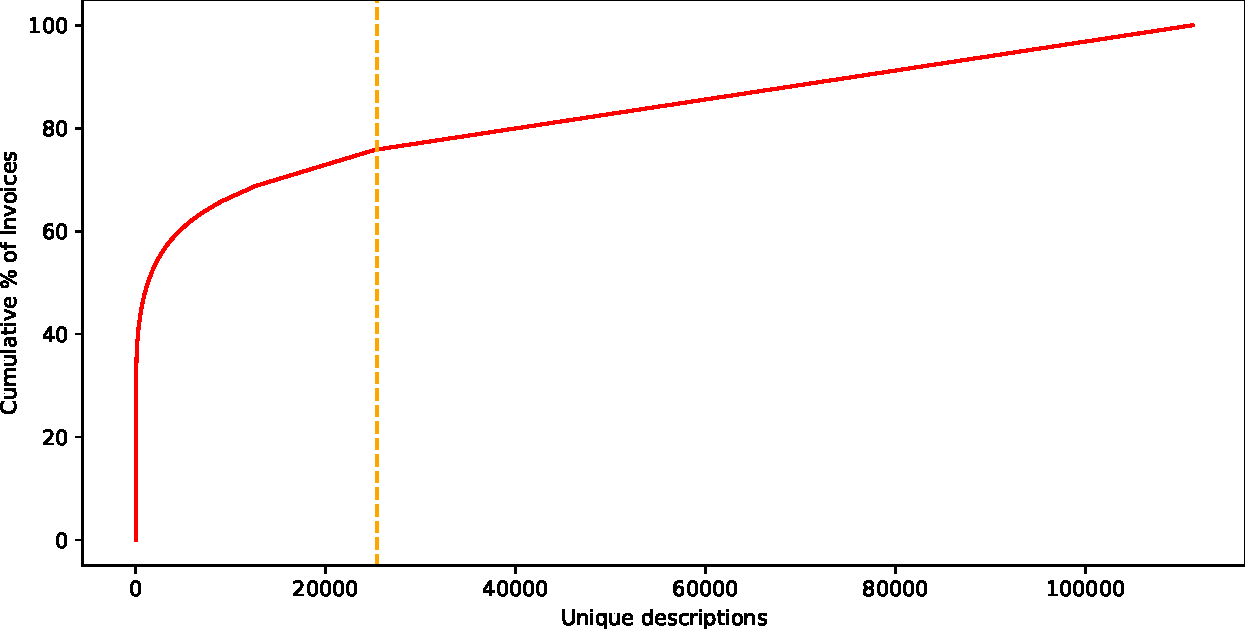
\includegraphics[height=6cm]{Bilder/data_understanding/descriptions_pareto.pdf}
	\caption{Percentage of Invoices by cumulative unique Descriptions}
	\label{fig:descr-hist}
\end{figure}
The frequency distribution of unique descriptions shows that the top third (36\%) of the descriptions covers 80\% of the invoices. It is notable, that the slope shows an edge at the point of the 24212the description. After this point, each following description only occurs once in the whole dataset. In turn, this means that only 20\% of the descriptions occur more than once.
\paragraph{Language Distribution}
The description of the invoices is related to the feature 'language', which describes the language of the invoice and its text fields. The most popular languages are English, Spanish, and German. It is noticeable, that there are over 700 languages or combinations of more than one language. 58878 invoices were not assigned a language, which is roughly one third of the total number.
\begin{figure}[h!]
	\centering
	\includegraphics[height=6.5cm]{Bilder/languages.pdf}
	\caption{Number of Invoices per Language}
	\label{fig:languages-bar}
\end{figure}

\begin{figure}[h!]
	\centering
	\includegraphics[height=6.5cm]{Bilder/languages_pareto.pdf}
	\caption{Percentage of Invoices by cumulative Number of Languages}
	\label{fig:languages-pareto}
\end{figure}


From the chart (\ref{fig:languages-pareto}) it can be inferred, that 80\% of invoices are in the top 16 languages. The slow rise after the top 80 languages indicates, that there are a lot of languages with a small number of invoices. This is also explained with a huge number of possible combinations of more than one language.


\paragraph{Invoice Item total Amount}
The invoice item total amount stands for the charge corresponding to one line in an invoice. Without very basic data cleaning, this column was not usable. The values were separated by a variety of different decimal delimiters and contained additional symbols. Also, the variation was initially very high due to some outliers in the magnitudes of $10^{217}$. Therefore, the values were aligned to one common decimal delimiter and stripped of the 1st and 99th percentile. This allows an initial insight into the distribution of the values.

\begin{table}[!h]
	\caption{Five-number summary for Item total Amounts}
	\centering
	\begin{tabular}{llllllll}
		\toprule
		 \textbf{mean} & \textbf{std. dev.} & \textbf{min} & \textbf{25\%} & \textbf{50\%} & \textbf{75\%} & \textbf{max} \\
		\midrule
		  4,749.69      & 17,687.85          & 1.64         & 45.84         & 276.20        & 1,520.00      & 197,721.71  \\
		\bottomrule
	\end{tabular}
\end{table}

The five-number summary shows that the values are skewed to the right in a considerable manner. The so-called tail of the price distribution reaches almost the 200,000 mark. For the further analysis, it will be interesting if very large charges belong into a similar group of spending.

\section{Data Quality}
In the analyses before several problems with the data could already be identified. Firstly, a lot of descriptions are empty or have the unusable value 'nan'. Secondly, the language distribution has shown that the spread is highly biased towards English. 
Both the unusable values and the uneven language distribution will be addressed in the data cleaning part of the thesis.

The quality of data for text mining purposes can be evaluated using four elementary dimensions \cite[p.~1279]{dataQualityAzeroual} :

\begin{table}[!ht]
	\begin{tabular}{lll}
		\vspace{0.5cm}
		\textbf{Completeness}                                                        & \begin{tabular}[c]{@{}l@{}}The extent to which data are of sufficient breadth, depth, \\ and scope for the task at hand\end{tabular}              &  \\
		\vspace{0.5cm}
		\textbf{Correctness} & The extent to which data is correct and reliable                                                                                                  &  \\
		\vspace{0.5cm}
		\textbf{Timeliness}                                                          & \begin{tabular}[c]{@{}l@{}}The extent to which the age of the data is appropriate \\ for the task at hand\end{tabular}                            &  \\
		\vspace{0.5cm}
		\textbf{Consistency}                                                         & \begin{tabular}[c]{@{}l@{}}The extent to which data are always presented in the same \\ format and are compatible with previous data\end{tabular} & 
	\end{tabular}
\end{table}

\paragraph{Completeness}
The invoices cover only a part of all billing documents received in the time frame. As a result, the analysis may not give an insight into the whole spending of one company but only into a fraction of it. 
Additionally, the data exploration has shown, that about one fourth of the descriptions are either empty or contain a placeholder for a missing value ('nan'). During data cleaning, even more unusable values will turn up. Still, a pessimistic estimate of 100,000 unique descriptions is a large enough dataset for telling analyses.

\paragraph{Correctness}
The data was created with the help of an annotation service. The vendor specializes on optical character recognition and \acf{NLP} to extract data from real documents, including invoices. Extractions results by this vendor have a guaranteed accuracy of 99\% \cite{scaleaiScaleDocumentAI}.
\paragraph{Timeliness}
The dataset consists of invoices in the time frame from 2015 to 2019, which makes it timely enough for the task.
\paragraph{Consistency}
 Annotations supplied by the annotation service always follow the given structure detailed in example \ref{code:JSONSchema}. This ensures consistency of data generated over a time span.
 
 To sum the data quality report up, the data has flaws in the dimension of completeness, but these minor issues with data quality will likely not impact further data analyses.
\chapter{Data Preparation}
    Data preparation is the process of transforming the acquired dataset into a dataset which can be fed into learning algorithms and is cleaned of impurities in such a way, that the learning results are likely satisfactory. Impurities to some extent were already identified in the prior chapter, additionally, shifted columns, encoding errors or different data formats have to be accounted for.
	Data preparation includes data wrangling, data cleaning, and feature extraction. What is left should be a uniform dataset, which is in a format that is understandable by the desired algorithms.
	
	\section{Data processing and data wrangling}

        \subsection{Alternatives}
        The chosen dataset consists of files in \ac{JSON} format. Several alternatives for storage and transforming the data exist. 
        
        \paragraph{Storage Location}
        Within the constraints of the thesis, three options are available for data storage. Firstly, data can be stored locally on the available machine. The data is available without internet access, and the local machine has high read/write speeds. This option requires no additional learning, and is free of charge for the department. A multitude of libraries exist for accessing files on a local file system. A downside is the limited scalability in terms of storage capacity and read/write operations. Additionally, local storage makes the data only available to this specific machine.
        
        Storing data on a cloud file sharing system is easy to operate and free of usage-bound charges. The storage space is virtually unlimited. Accessing files on sharing platforms is feasible but tedious. The access can be shared within the company context, but everyone is subject to the limited accessibility. Using a files storage service could be of use for transferring data without a physical connection. Still, this is the only recommended use case in this context.
        
        The third option is storing the data using a specialized storage service, such as AWS S3. While the learning overhead is higher in the beginning, the scalability is a convincing argument. Billing is according to usage, but adequate because of the high connectivity with other cloud-based ML service offerings inside and outside of SAP.
        
        \begin{table}[ht]
            \centering
            \caption{Comparison of available Storage Options}
            \begin{tabular}{clll}
                \toprule
                &\textbf{Local} & \textbf{Cloud Filesharing} & \textbf{Specialized Storage Services} \\
                \midrule
                
                Example     & \begin{tabular}[c]{@{}l@{}}2.6GHz \\ 512GB SSD\end{tabular} & Microsoft OneDrive                                                        & AWS S3                                                                                                 \\
                \midrule
                Ease of use & high                                                        & high                                                                      & higher learning overhead                                                                               \\
                \midrule
                Cost        & free of charge                                              & free of charge                                                            & \begin{tabular}[c]{@{}l@{}}billing according to \\ used storage space\end{tabular}                     \\
                \midrule
                Scalability & limited                                                     & unlimited                                                                 & unlimited                                                                                              \\
                \midrule
                Data access & local                                                       & \begin{tabular}[c]{@{}l@{}}limited remote \\ access capacity\end{tabular} & \begin{tabular}[c]{@{}l@{}}local, remote, high \\ connectivity to \\ ML service offerings\end{tabular}\\
				\bottomrule
                
            \end{tabular}
            \label{tabelle:storage}
        \end{table}
        
        \paragraph{Data Format}
        The data is still available only in the from \ac{JSON} documents. Python allows for easy parsing of these objects, but this option is highly inefficient compared to native Python data structures.
        The equivalent to \ac{JSON} in Python are combinations between lists and dictionaries. Dictionaries are an implementation of the \lstinline|Map| data structure.
        
        This option stands in contrast to a data format commonly used in data science tasks: the \lstinline|DataFrame|. Both formats, the dictionaries and DataFrames have specific advantages and disadvantages.
        
        The \lstinline|DataFrame| is structured like a table, consisting of labeled rows and columns. This data structure is implemented in the library \lstinline|pandas|. 
        Different data formats such as strings, floats or boolean values can be stored in the table.        Optimized methods for calculating row-wise and column-wise operations are supplied in the library. This makes the \lstinline|DataFrame| one of the most popular tools for data scientists.
        
       \lstinline|DataFrame|s being suited for various purposes, makes them inflated and slower than low-level data structures. The indexing operation, for example, has to address a multitude of cases. This makes it slower than a simple dictionary access. Appendix \ref{benchmarkDF} details the comparison in a benchmark.
       
       Surprisingly, storing \ac{JSON} data in a \lstinline|DataFrame| is less memory-intensive than storing the same data in dictionaries and lists \cite{DFvsJSON}. This means  \lstinline|DataFrame|s are favorable for storage and calculations with large data quantities.
       
       Considering all factors, the best choice is transforming the dataset into a  \lstinline|DataFrame|. Still, the advantages of dictionaries and lists in basic use-cases will be kept in mind for later.
     
    \subsection{Theoretical Implementation}
    For the data wrangling the invoices have to be read into memory and then processed into a reusable structure. All invoices will be combined into \lstinline|DataFrame|s, which then are persisted for later use.
	
    \begin{figure}[ht]
        \centering
        \includegraphics[height=5cm]{Bilder/practical/entity_relationship.png}
        \caption{Entity Relationship Diagram for Invoice Documents}
        \label{fig:er}
    \end{figure}
	The documents can be separated into two fundamental entities: the invoice and the line items. The entity relationship diagram (\ref{fig:er}) shows how invoices and line items are related. The invoice contains at least one line item, and the information in the invoice is relevant to all of its line items. This includes information about the vendor, and the invoice date. The line items of an invoice contain specific information on the products, such as the material number and the description.
	An invoice and its line items can be matched through an unique identifier, which is also the filename.

	 \begin{figure}[ht]
		\centering
		\includegraphics[height=11.5cm]{Bilder/preprocessing/df_schema.png}
		\caption{Theoretical Implementation of the Data Wrangling}
		\label{fig:invoice_df_schema}
	\end{figure}	

	Now, looking at the technical side of the file composition.	The data for an invoice and its line items is stored in an array of objects. The array "annotations" contains objects, each one representing information such as the invoice date or the unit price. A schematic description of how the invoice data should be represented after extraction is shown in Figure \ref{fig:invoice_df_schema}: One invoice is modeled as one row in the table. Different attributes are represented as columns.
	Information about line items have labels containing the prefix "lineItem". One invoice containing several items is represented by duplicate values of one label (in the example \ref{fig:invoice_df_schema} the label "lineItem.description.value"). Each new label "lineItem.description.value" denotes a new line item. Here, the order of the labels has to be retained during data wrangling to ensure not mixing up information about different invoice items. Each new line item should be a new row in the table of line items.
	
	The goal of the data wrangling process is to create two \lstinline|DataFrame|s, one for the invoices and one for the line items.
	Additionally, another data structure will be created to optimize recurring and complex operations.
	
	Data exploration shows, there are only 79.741 unique descriptions for the listed items. By saving only the unique values, the required space is reduced to less than one fourth compared to before. Additionally, this step is required by most machine learning models, as duplicate input values can skew the outcome. The model is chosen later, so this processing step leaves the model selection more open to different kinds of learning algorithms.
	
	After the deletion of duplicate descriptions, the relationship between one line item and its description is not one-to-one, but rather one description belonging to several different line items. Model outputs will be a classification of one description, so to restore the relationship between the classification result and one line item, a mapping is constructed.
	This dictionary maps one description to all line items (more specifically, their ID) with this description.
	\begin{figure}[ht]
		\centering
		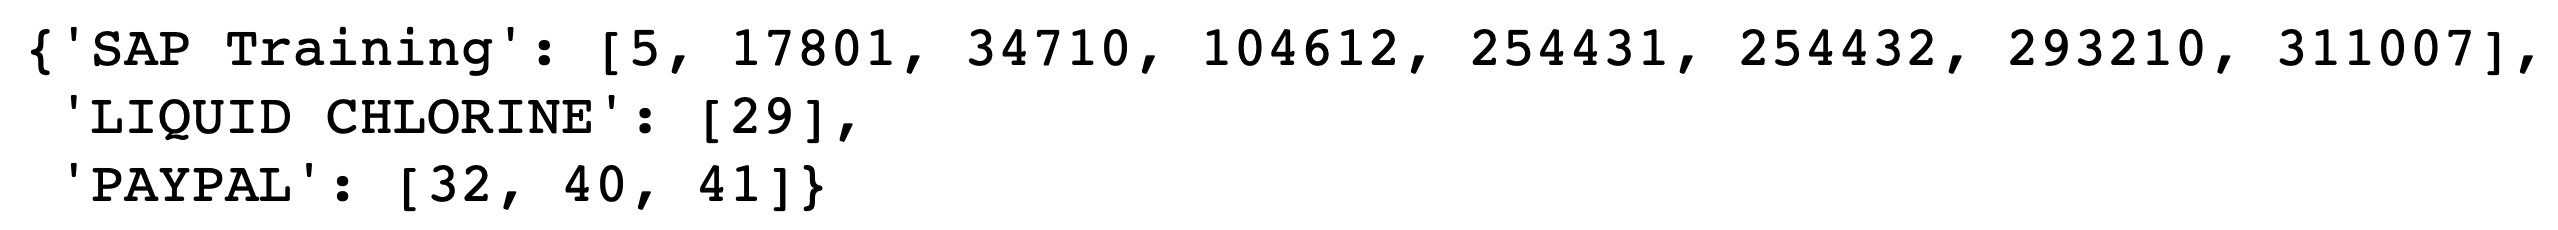
\includegraphics[width=\linewidth]{Bilder/description_map.png}
		\caption{Mapping Descriptions to their Line Item IDs}
		\label{fig:mapping}
	\end{figure}


	After the construction of both tables and the mapping, these artifacts should be serialized. This way, they can easily be loaded into memory without the effort to reconstruct them from scratch.
	
    \subsection{Practical Implementation}
	
	The files were processed using a Python script (\ref{code:InvoiceReader}). The information on invoices is stored in a tabular data structure, a \lstinline|pandas DataFrame|. Worth mentioning is that some invoices contain more information than others. In this case, invoices are still appended into one table, but fields for non-existent values are left empty. In Figure \ref{fig:df-invoices}, the first invoice does not have a total amount included, but since the second one does, this column is created.
	The filename of one invoice contains the unique identifier for one invoice.
	
	\begin{figure}[ht]
		\centering
		\includegraphics[height=2.5cm]{Bilder/practical/df_invoices.png}
		\caption{Exemplary depiction for processed invoices in a DataFrame}
		\label{fig:df-invoices}
	\end{figure}

	Similarly, information on the invoice items is retrieved from the documents and stored in a \lstinline|pandas DataFrame|. Every line item has an unique id and can also be linked to the respective invoice through the filename.
	
	\begin{figure}[ht]
		\centering
		\includegraphics[height=6cm]{Bilder/practical/df_lineitems.png}
		\caption{Exemplary depiction for processed invoice items in a DataFrame}
		\label{fig:df-invoice}
	\end{figure}
	
	The resulting two \lstinline|DataFrame|s are serialized with the Python standard library \lstinline|pickle|. The data can be efficiently loaded into memory and re-serialized again with this library.
	
	This processing step allowed for storing the initial 5.12GB of data in a more usable format and takes up only a total of 393MB.

	The process of reading files from the disk is not inherently an expensive one, but in the realms of many thousand documents, processing times soon reach several days. Observing the execution of the Python code showed a peculiarity: While the utilization of the used processor was consequently at the maximum (in Figure \ref{fig:cpu} at 97.1\%), only one process is executed, leaving the total \ac{CPU} usage at only 20\%. 
	
	\begin{figure}[ht]
		\centering
		\includegraphics[height=5cm]{Bilder/practical/python_processes.png}
		\caption{\acs{CPU} Usage during single-process Python Execution}
		\label{fig:cpu}
	\end{figure}
	
	
	One question that may now arise is: Why doesn't Python split up the workload and employ the full capacity of the machine?
	This can be explained with the design of the Python interpreter. The Global Interpreter Lock controls access to the Python Virtual Machine executing the code. This lock only allows exactly one thread to run at a time \cite[ch.~18.3.1]{corePython}. This of course is not favorable, as valuable CPU capacity is idle. Fortunately, the lock behaves in a special way regarding C routines: the lock is released before executing C code \cite[ch.~18.3.1]{corePython}. I/O operations in Python, such as opening files, utilize C code. This allows to bypass the, in this case, inconvenient locking mechanism. 
	
	Different Python libraries exploit this specialty and allow to spawn a pool of different processes, which then execute calls asynchronously. The \lstinline|ProcessPoolExecutor| is one example of multiprocessing.
	
\begin{lstlisting}[language=python, 
label=code:process-pool,
caption=Spawning a Process Pool in Python,
style=EigenerPythonStyle]   
with concurrent.futures.ProcessPoolExecutor() as executor:
	results = process_map(r.read_invoice, filenames, chunksize=2000)
\end{lstlisting}

	The \lstinline|ProcessPoolExecutor| (s. listing \ref{code:process-pool}) can distribute a list of input values for functions (\lstinline|filenames| ) onto a function (\lstinline|r.read_invoice|). Additionally, the \lstinline|chunksize| as parameter specifies how large the bundles of input values for each process are. Distributing the workload onto all \ac{CPU} cores, the processing time was reduced from 27 hours to under 4 minutes. 
	
	\section{Data cleaning}
	Data cleaning concerns removing all impurities from the data. This includes deleting duplicates, using an uniform data type, and removing unnecessary information.
	Just the descriptions of all the line items will be fed into models, therefore only those have to be cleaned. The Python library \ac{NLTK} provides useful methods for cleaning textual data.
	
	\lstinputlisting[
	label=code:cleaner,    % Label; genutzt für Referenzen auf dieses Code-Beispiel
	caption=Python Script for extracting JSON Data into a DataFrame,
	captionpos=b,               % Position, an der die Caption angezeigt wird t(op) oder b(ottom)
	style=EigenerPythonStyle,   % Eigener Style der vor dem Dokument festgelegt wurde
	firstline=0,                % Zeilennummer im Dokument welche als erste angezeigt wird
	lastline=23                 % Letzte Zeile welche ins LaTeX Dokument übernommen wird
	]{Quellcode/cleaner}
	
	In the code example \ref{code:cleaner}, the text is firstly separated into tokens. Then each token is examined whether it contains non-alphabetic characters. Only alphabetic tokens are retained. Again, this process is highly computationally intensive due to the size of the data. Therefore, this task was completed using the same procedure for multiprocessing as detailed in the prior section.
	
\begin{lstlisting}[
	language=sh,
	caption=A Description before and after Data Cleaning,
	label=code:cleaned_descr
	]
$ python3 -c 'import cleaner; print(cleaner.clean("500grams of special baking flour type 504"))' \\
>>>  ['of', 'special', 'baking', 'flour', 'type']
\end{lstlisting}
	 
	 The code example \ref{code:cleaned_descr} shows the input and output of this procedure. A token is completely discarded if it contains non-alphabetical characters, as these tokens are more than often not an accurate descriptor of the text's meaning.	

        
        \section{Feature Extraction and Feature Engineering}
        \label{section:feature-extraction}
        The majority of popular \ac{ML} algorithms require the input of scalar, vector or matrix data. Several methods for representing text as mathematical object will be discussed in the following.
    
            \subsection{Alternatives}
            Firstly, the distributional representations will be explained and evaluated.
            
            \subsubsection{Term-Document Incidence Matrix}
			\label{section:tdim}
            \begin{figure}[h]
            	\centering
            	 \includegraphics[height=3.5cm]{Bilder/corpus_bow.png}
            	\caption{Example Corpus}
            	\label{fig:term-doc-incidence}
            \end{figure}
            The three documents in Figure \ref{fig:corpus} will be considered to explain the workings of the one-hot encoding. A corpus is transformed into a term-document incidence matrix representation in two steps. 
            
            \begin{figure}[h!]
            	\centering
            	\includegraphics[height=2.5cm]{Bilder/preprocessing/term-document-incidence.png}
            	\caption{Term-Document Incidence Matrix}
            	\label{fig:corpus}
            \end{figure}
            
            Firstly, the vocabulary is determined. 
            It is a collection of all words occurring in the corpus. Every word is contained exactly once, regardless of the actual number of occurrences. The vector representation of one document is of the same length as the vocabulary. One document being represented by one vector, a corpus of several documents can be represented as a matrix. The resulting matrix $M$ has the size $ |D|*|V| $, with $|D|$ being the number of documents in the corpus, and $|V|$ being the size of the vocabulary.
            
            Secondly, for each combination of one document $ d_{i} $ and one word $ v_{j} $ in the vocabulary, it is determined whether the word occurs in the document. This information is encoded binary with a "1" at $m_{ij}$ for occurrence and a "0" for no occurrence. The resulting vectors for the three documents are:
            \[ d_{1} = [0,1,0,0,0,1,0,0] \]
            \[ d_{2} = [1,0,1,0,1,0,1,1] \]
            \[ d_{3} = [0,0,0,1,0,0,0,1]\]
    		The drawback of this method is that no consideration is paid to words being repeated in one document. Additionally, no semantic relationship between words or documents can be inferred. 
    		Further, it can be stated, that the \ac{BoW} representation fails to capture the meaning of synonyms. This becomes obvious with an example: document $ d_{1} $ and $ d_{3}$ would be considered to belong into the topic of transportation or automotive. The \ac{BoW} representation suggests topical proximity between document $ d_{2} $ and $ d_{3}$ , through the shared word "ticket". "Ticket" here is used in both the meaning of an entrance pass ($d_{2}$) and in the meaning of a note for a traffic offense  ($d_{3}$). 
    		Further, this feature extraction method strongly suffers from high dimensionality \cite[ch.~3.2]{practicalNLP}, since the matrix dimensions depend on the size of the vocabulary. 
    
            \subsubsection{Bag of Words Model}
 			With the \ac{BoW} model, the only difference to a term-document incidence matrix is that the occurrences of a word are counted, instead of a binary encoding.
             \begin{figure}[ht]
            	\centering
            	\includegraphics[width=\textwidth]{Bilder/bow.png}
            	\caption{\acl{BoW} Representation of Documents}
            	\label{fig:bag-of-words}
            \end{figure}
            
            The result of vectorization are three vectors:
            \[ d_{1} = [0,1,0,0,0,1,0,0] \]
            \[ d_{2} = [1,0,1,0,1,0,1,2] \]	
            \[ d_{3} = [0,0,0,1,0,0,0,1]\]
            
            \subsubsection{Tf-Idf}
            \label{section:tfidf}
            The \ac{TF-IDF} model aims to capture more meaning from the corpus by considering the composition of the whole corpus for the calculation of individual document vectors. \ac{TF-IDF} makes two assumptions about natural language:
            \begin{enumerate}
            	\item A word $t_{i} $ which occurs very frequently in one document is considered to describe a text very well (term frequency).
            	\item A word $t_{i} $ which occurs in a large number of documents does not describe one document well (inverse document frequency).
            \end{enumerate}
            
            \subparagraph{Term Frequency}
            The occurrences of one word in one document is denoted as $ \#( t_{i}) $.
            One additional consideration needs to be made regarding the document length. In a document of length $ |d_{2}| = 6 $ and a document of length  $ |d_{3}| = 2 $, the word $ t_{i} $occurring once should be considered more important to $ d_{3} $, since it accounts for a larger share of the text. The measure resulting from this idea is the term frequency:
            
            \[ TF(t_{i}, d_{j}) =   \dfrac{\#( t_{i})}{|d_{j}|} = \dfrac{occurences \; of \; word \; t_{i} \: in \; document \;\:   d_{j}}{legth \; of \; d_{j}} \]
            
            \subparagraph{Inverse Document Frequency}
            Words occurring in many documents often are articles or pronouns (stop words) which do not provide value when inspecting the content of a text. The inverse document frequency is a measure accounting for this fact. The inverse document frequency of a word is the proportion between the number of documents in the corpus and the number of documents containing the word. The logarithm is applied, as the importance of a word does not increase proportionally to the number of occurrences.
        
            \[ IDF(t_{i}, d_{j}) = \log \dfrac{|D|}{\#(d_{t_{i}}) } =  \log \dfrac{number \;  of\;  documents \;  in \; corpus \; D}{ number \; of \; documents \; containing \; word \; t_{i}} \]
            
            Combining both assumptions, the \ac{TF-IDF} measure is created:
             \[ TFIDF(t_{i}, d_{j}) \;=\; TF(t_{i}, d_{j}) * TF(t_{i}, d_{j})\]
            
            For the corpus displayed in the previous section the document vectors calculated with the \ac{TF-IDF} measure are:

           \begin{table}[!h]
           	\centering
           	\begin{tabular}{llllllllll}
           		$d_1 = [$ & 0.     & 0.7071 & 0.     & 0.     & 0.     & 0.7071 & 0.     & 0.     & $]$ \\
           		$d_1 = [$ & 0.3979 & 0.     & 0.3979 & 0.     & 0.3979 & 0.     & 0.3979 & 0.6053 & $]$ \\
           		$d_1 = [$ & 0.     & 0.     & 0.     & 0.7959 & 0.     & 0.     & 0.     & 0.6053 & $]$
           	\end{tabular}
           \end{table}
                
            The \ac{TF-IDF} measure corrects some of the pitfalls of the \ac{BoW} model. It certainly is less vulnerable to skewing by stop words,  as words are ranked by importance to each document and the all over corpus. 
            
        
            The above mentioned methods are distributional representations \cite[ch.~3.3]{practicalNLP}. They all suffer from similar problems. The vectors contain one element for each word in the vocabulary, resulting in vectors which are high-dimensional and very sparse. Also, \ac{TF-IDF} fails to represent the topical relationship between $ d_{1} $ and $ d_{3}$. Finally, these methods can not handle an inference for words which are not in their vocabulary \cite[ch.~3.2]{practicalNLP}.
            
            Following methods are distributed representations. They are designed to alleviate the drawbacks of distributional word representations.
            
            \subsubsection{Word Embedding BERT}
             The most desirable vector representation consists of dense low-dimensional vectors which are close to each other if the words are considered similar. The lack of understanding of related words, and the problem of high-dimensionality is corrected with the third presented option: word embeddings.
            
            An embedding is a translation of a word into a high-quality vector. The model does so, as it has been trained on a large set of natural language data. The first model for continuous vector representations was word2vec \cite{word2vec2013}. Being published in 2013, the model has been already replaced by new state-of-the-art models such as \acs{BERT}. This new model builds on the premised of word2vec, but was able to obtain astonishing results at tasks such as answering questions using the Stanford Question Answering Dataset \cite[p.~6]{BERT}. 
            
            The \ac{BERT} model can represent unlabeled text by learning on large textual corpora. Its name is assembled from its different components:
            
			\begin{table}[!h]
				\begin{tabular}{lll}
					\vspace{0.5cm}
					B & Bidirectional   & \begin{tabular}[c]{@{}l@{}}The model considers both left context (previous words) and \\ the right context (following words) during learning.\end{tabular}        \\
					\vspace{0.5cm}
					E & Encoder         & The model consists of several encoder layers.                                                                                                                     \\
					\vspace{0.1cm}
					R & Representations & \begin{tabular}[c]{@{}l@{}}Sequence representations are a projection of a sequence \\ onto a vector which is able to reflect the sequence's meaning.\end{tabular} \\
					\vspace{0.1cm}
					& from            &                                                                                                                                                                   \\
					\vspace{0.1cm}
					T & Transformers    & \begin{tabular}[c]{@{}l@{}}BERT belongs into the family of transformer models and \\ utilizes parts of the transformer architecture.\end{tabular}                
				\end{tabular}
			\end{table}

           
           The model is trained on two tasks. Firstly, it is trained on word prediction (\ref{fig:mlm}). \ac{BERT} had to predict one missing word in a text unit. The objective of course is to get the right word. The loss in this task is measuring if and how wrong a prediction is. The second task is to predict the next sentence after a text section. The objective is to predict the correct words and their order. The model is trained by adjusting internal weights in such a way, that both losses are minimized. In turn this means, the model can predict missing words and next sentences with minimized error.
           
          
             \begin{figure}[h!]
             	
             	\centering
             	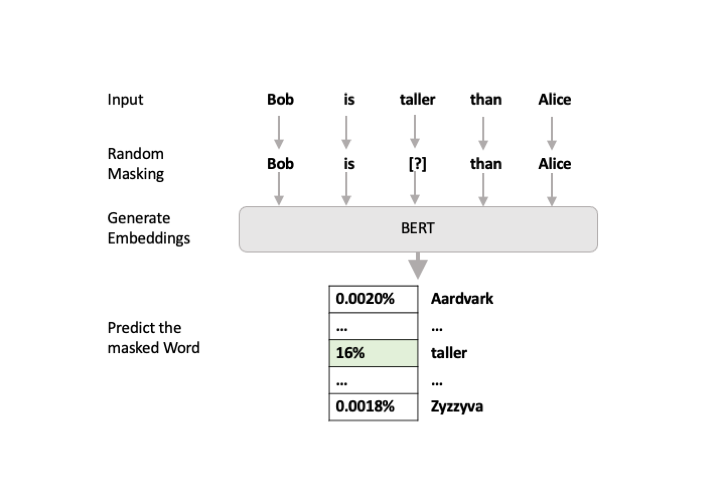
\includegraphics[height=10cm]{ Bilder/preprocessing/BERT/BERT-language-modeling-masked-lm.png}
             	\caption[Training BERT with the MLM task]{Training BERT with the MLM task \cite{alammarIllustratedBERTELMo}}
         		\label{fig:mlm}    
         \end{figure}
            
         
               BERT is trained with millions of Wikipedia articles, meaning the inputs is a large text database. The text segment is split into tokens, which are then encoded as a vector of length 768 \cite[p.~3]{BERT}. Next follows the positional encoding. When applying the transformer encoder to a sequence of words, the output should be dependent of the sequence of the input words. E.g. the sentences "Bob is taller than Alice" and "Alice is taller than Bob" should be encoded as two different vectors. This can be realized with encoding the position of each token. 
               

               
               The token embedding and its positional encoding are now added, and fed into the encoder \cite{illustratedTransformer}. Inside the encoder, four elements process the input sequentially:
               
               \begin{enumerate}
               	\item The self-attention mechanism allows for the model to incorporate the context of a token into its encoding. The mechanism does so by calculating the importance of inputs with themselves ("self") and returns which tokens are important to each other's meaning ("attention").
               	\item To reduce the computational requirements for training a deep neural network, the layers of neurons in the networks are normalized with respect to their activation. This reduced the training time while not impacting the result, which is only dependent on the learning algorithm \cite[p.~10]{baLayerNormalization2016}.
               	\item The \ac{FFNN} takes the results of the layer normalization and the residual connection as input. When the whole transformer is trained on a specific task, the parameters (weights) of this model are also trained. Therefore, the \ac{FFNN} is one gear in the whole process of reaching the transformer's task.
               	\item Finally, the results are normalized again.
               \end{enumerate}
       			
       			 \begin{figure}[h!]
       				\label{fig:encoder}
       				\centering
       				\includegraphics[height=7cm]{Bilder/preprocessing/BERT/encoder.png}
       				\caption[The Transformer Encoder Architecture]{The Transformer Encoder Architecture  \cite{illustratedTransformer}}
       			\end{figure}
			
            
            Evaluating all different models for word vectorization, BERT clearly outperforms the distribustional representations:
            \begin{itemize}
            	\item Word embeddings produce dense and lower-dimensional vectors than distributional representations.
            	\item With word embeddings, the resulting vectors perform a lot better on common \ac{NLP} tasks, meaning the resulting vectors are of higher quality than with distributional representations.
            	\item BERT can process out-of-vocabulary words, this is a big advantage to previous embeddings.
            \end{itemize}

			The advantage of BERT over the other presented options is obvious. But, now there are two unconsidered restrictions:
			First, BERT only encodes words.
			Second, BERT is only in one language.
			
			Luckily, researchers around BERT encountered similar tasks and developed a new BERT model to solve this. 
			First, the Sentence-BERT embeddings are generated in a way that requires only minimal additions to the BERT architecture \cite[p.~2]{sentenceBERT}. Sentence-BERT is trained with a dataset of sentences, labeled with their relationship (contradiction, entailment, neutral) \cite[p.~4]{sentenceBERT}. Two sentences each pass through a BERT model. A pooling layer for each of the two calculates a weighted sum of all words in the sentence to create the embedding for the whole sentences. With the labels and the comparison of two sentence embeddings, the pooling layer is trained. The weights in both pooling layers are adjusted over time, creating a so-called Siamese Network.
			
			Secondly, the embeddings need to be able to understand different languages. A multilingual implementation of BERT can solve this. A multilingual embedding should align vectors in different languages in such a way, that translated sentences are very close in the vector space. A multilingual Sentence-BERT model trains on a dataset with sentences and their translation \cite[p.~2]{mBERT}. The weights in the BERT model are adjusted by completing the task of assigning the same sentence in different languages a similar vector \cite[p.~2]{mBERT}.
			
			Both the multilingual and sentence embeddings require very little additional complexity compared to the underlying BERT model. But, these additions help to accurately represent the content in the dataset.
			
            \subsection{Theoretical Implementation}
            
           	After explaining and evaluating the alternatives, the most favorable one, the word embeddings using \ac{BERT} will be put into practice. In theory, a BERT model would have to be trained using a large text dataset. This took the developers of BERT at Google 4 whole days, and required 4 \ac{TPU}s \cite{BERTTraining}. Fortunately, the researchers published this trained model, making it free to use for the public \cite[p.~2]{BERT}.
            	
            From the available pre-trained models, the \lstinline|distiluse-base-multilingual-cased| model fulfills all the requirements (sentence embeddings, multilingual vector alignment). The prefix 'distiluse' stands for distilled universal sentence encoder, meaning the sentence encoder is compressed in a model with a more portable size. The suffix 'cased' means that words are handled case-sensitive.
            
            Since the description data has already been transformed into a usable format and cleaned, the descriptions can now easily be fed into the \lstinline|distiluse-base-multilingual-cased| model.
            	
            \subsection{Practical Implementation}
             
             The model can be laded using the library \lstinline|sentence_transformers|. The library can create a model from the name of the transformer. Embeddings can be generated very easily, and are returned as a 2D-array. This inference takes about 30ms. For all 79.741 documents, this means an total time of about 40 minutes.
             
\begin{lstlisting}[language=python,
	label=code:generate-embed,
	caption=Generating an Embedding with BERT,
	style=EigenerPythonStyle]   

from sentence_transformers import SentenceTransformer
model = SentenceTransformer(
	'sentence-transformers/distiluse-base-multilingual-cased-v2'
	)
sentence = ["Service Charge for Flight FRA-LAX"]
embedding = model.encode(sentence)
print(embedding)
>>> 	[[-0.02105838 -0.01305696 -0.0403975  ...  0.08315323  0.06774105  0.03354893]
\end{lstlisting}

		Since data cleaning and data wrangling could be sped up significantly with multiprocessing, it stands to reason that this might also work for the inference on BERT. Batching and parallel processing only provides a speed-up if the model can utilize a strong \ac{GPU} \cite{schopfParallelInferenceHuggingFace2022}. This is not the case, so we settle with a one-time processing taking 40 minutes.
		
		During processing, the hardware was overheating and shutting down. To prevent losing progress, batches of 1000 documents were processed at a time, serialized and written on the hard disk. Upon completion, the files are loaded into memory again and unified into one collection of 20MB in vectors.

		These vectors are now ready for clustering.            
\chapter{Modeling}
The objective of this thesis is the grouping of expenses with the methods of \ac{NLP}. Grouping, or clustering, is the practise of sorting data points into groups in such a way that the similarity inside a group (intra-cluster similarity) is high while the similarity between clusters (inter-cluster similarity) is low. The defintion of similarity as well as different clustering algorithms are presented and contrasted in the following sections.


\section{Alternatives}
\subsection{Similarity and Distance Measures}
A distance measure is a quantification of how near objects in space are. Distance measures can be defined for spaces of arbitrary numbers of dimensions. In the examples, four words (man, woman, king, queen) are compared in their semantic similarity. The word vectors were generated with a word embedding, but the focus is on comparing the distance measures available for clustering later on.

		\begin{figure}[!h]
			\centering
			\includegraphics[height=6cm]{Bilder/models/heatmap_dot_product.pdf}
			\caption{Dot Product as Similarity Measure}
			\label{fig:dotproduct-heatmap}
		\end{figure}
	
		\subparagraph{Dot Product}
		The dot product is an operation transforming a vector into a scalar through multiplying the vectors element-wise. This operation is easily and efficiently calculated, but has some pitfalls.
		While every word in the example \ref{fig:dotproduct-heatmap} ranks very high in similarity to itself, the distance between the word and itself is not always the same for every word. This happens because the dot product is not agnostic of a vector's magnitude. A vector's product with itself is the square of its magnitude. This results in the similarity of man-man to be lower than the similarity of queen-queen.
		This fact makes the dot product impractical for accurately representing the relationships of words.
	
					\[ 
				\text{dot product} :=  \mathbf{A} \cdot \mathbf{B}= \sum\limits_{i=1}^{n}{A_i  \mathbf{B}_i} 
				\]

	
		\subparagraph{Euclidean Distance} \label{euclidean}
		For low-dimensional applications, this distance works well and shows great results. Euclidean distance can be calculated in a highly efficient manner, even for n dimensions \cite[ch.~6.2]{40algorithms}. This suggests, that euclidean distance is particularly suitable for high-dimensional data. Unfortunately, euclidean distance falls victim to the curse of dimensionality. In \cite[p.~1]{beyerNearestNeighbor} it is proven that with increasing dimensions, the distance between data points approaches an uniform value for all data points. This effect could be demonstrated for spaces with as little as ten dimensions. Therefore, it can be said that euclidean distance is not suitable for high-dimensional data. With vectors in \ac{NLP} ranging from 100 to 800 dimensions with embeddings and hundreds of thousands with \ac{TF-IDF}, this distance measure is not suitable.
		
				\[ 
		\text{euclidean distance} :=  \sum\limits_{i=1}^{n}{(A_i -  \mathbf{B}_i)^{2}} 
		\]
		
		\begin{figure} 
			\begin{minipage}{0.49\textwidth}
				\label{fig:euclidean}
				
				\includegraphics[height=5cm]{Bilder/models/euclidean}
				\caption{Euclidean Distance as Measure}
			\end{minipage}
			\hfill
			\begin{minipage}{0.49\textwidth}
				\includegraphics[height=5cm]{Bilder/models/cosine}
				\caption{Cosine Similarity as Measure}
				\label{fig:cosine}
			\end{minipage}
			\hfill
		\end{figure} 
	
		\subparagraph{Cosine Similarity}
		The name of this measure already suggests that not distance but similarity of objects is measured. Instead, it quantifies how close two vectors are [ch.~6.1.2].  Mathematically, the cosine distance is the cosine of the angle between two vectors. A wide angle means a high distance between two vectors, or in this case two words [ch.~6.1.2]. Narrow angles stand for a low distance and words being closely related. In example \ref{fig:cosine}, the word vectors for woman and king have a higher angle than those of woman and queen. This means the words woman and queen are more similar thank woman and king.
		
		\[ 
		\text{cosine similarity} := \cos(\theta) = {\mathbf{A} \cdot \mathbf{B} \over \|\mathbf{A}\| \|\mathbf{B}\|} = \frac{ \sum\limits_{i=1}^{n}{\mathbf{A}_i  \mathbf{B}_i} }{ \sqrt{\sum\limits_{i=1}^{n}{\mathbf{A}_i^2}}  \sqrt{\sum\limits_{i=1}^{n}{\mathbf{B}_i^2}} }
		  \]
		
		The difference between cosine distance and euclidean distance is clear: cosine measures the angle, and euclidean the vector length. But which one performs better in high dimensions? Cosine distance is perceived as more suitable for high dimensional data \cite[ch.~6.2]{40algorithms}, and often suggested for \ac{NLP} tasks. 
		
		But there is one fact left out in this suggestion: On normalized data (all vectors are unit vectors), cosine distance and euclidean distance are linearly connected \cite{khanRelationshipCosineSimilarity2020}.
		
		\begin{align*}
			\cos(\theta_{AB}) &= {\mathbf{A} \cdot \mathbf{B} \over \|\mathbf{A}\| \|\mathbf{B}\|}  \\
			\\
			\text{For normalized vectors with } \|\mathbf{A}\| &=1 \text{ and } \|\mathbf{B}\| =1 \text{ this equals to}: \\
			\cos(\theta_{AB}) &=  {\mathbf{A} \cdot \mathbf{B} \over 1 * 1 } = \mathbf{A} \cdot \mathbf{B}
		\end{align*}
		
		\begin{align*}
			d(\mathbf{A}, \mathbf{B}) &:=  \sum\limits_{i=1}^{n}{(\mathbf{A}_i -  \mathbf{B}_i)^{2}} \\
			&= \sum\limits_{i=1}^{n}{\mathbf{A}_i^{2} - 2\mathbf{A}_i\mathbf{B}_i + \mathbf{B}_i^2}  \\ 
			&= \sum\limits_{i=1}^{n}{\mathbf{A}_i^{2}} + \sum\limits_{i=1}^{n}{- 2\mathbf{A}_i\mathbf{B}_i} + \sum\limits_{i=1}^{n}{\mathbf{B}_i^2} \\
			&= 	\|\mathbf{A}\| + \sum\limits_{i=1}^{n}{- 2\mathbf{A}_i\mathbf{B}_i} + \|\mathbf{B}\| \\
			&= \|\mathbf{A}\| -2 \sum\limits_{i=1}^{n}{\mathbf{A}_i\mathbf{B}_i} + \|\mathbf{B}\| \\
			&= \|\mathbf{A}\| -2 (\mathbf{A} \cdot \mathbf{B}) + \|\mathbf{B}\| \\
			\\
			\text{For normalized vectors with }\|\mathbf{A}\| &=1 \text{ and } \|\mathbf{B}\| =1  \text{ and } \mathbf{A} \cdot \mathbf{B}  = \cos(\theta_{AB}) \text{ this is equal to}:\\
			d(\mathbf{A}, \mathbf{B}) &= 1 - 2 \cos(\theta_{AB}) + 1 = 2 - 2(\cos(\theta_{AB}))
		\end{align*}
		Both solutions are linear to each other: $2 - 2(\cos(\theta_{AB})) \sim \cos(\theta_{AB})$.
	
		Now, with the newly gained insight into the distance relationships of normalized vectors of $\cos(\theta_{AB}) = \mathbf{A} \cdot \mathbf{B}$ and $d(\mathbf{A}, \mathbf{B}) = 2 - 2(\cos(\theta_{AB}))$ , it can be stated that the cosine distance and euclidean distance of two normalized vectors are linearly related.
				
		Cosine and euclidean distance being connected linearly for normalized data has not made the decision easier. But there is an additional factor: 
		Algorithms often require distance metrics to obey the four requirements of a metric space \cite[p.~32]{schubertTriangleInequalityCosine2021}.
		These requirements are \cite[p.~22]{rajaramanNeighborSearchHigh}:
		\begin{enumerate}
			\item The distance between to points is 0 if and only if they are identical.
			\item The distance between two points is never negative.
			\item The distance is equal irrespective of the starting point.
			\item The shortest distance between two points is a straight line.
		\end{enumerate} 
		
		All aforementioned arguments make a strong case for the euclidean distance.
		
\subsection{Clustering Algorithms}
		
		\subparagraph{K-Means}
		The k-Means algorithm generates $k$ groups of data by iteratively adapting clusters and their centers. In the first iteration, the $k$ cluster centers are chosen randomly. Each point in the dataset is assigned to its nearest cluster center. The cluster centers for the next iteration are now the mean values of all points in one cluster. The process of reassigning and calculating the mean is repeated until the cluster centers don't change.
		
		The algorithm is mainly focused on performance, hence the design is kept lean by omitting logic for determining the number of clusters \cite[ch.~6.2]{40algorithms}. Following pseudo code illustrates the workings of the algorithm.
		
%		\begin{lstlisting}
%randomly choose k_centers
%while (iterations < max_iterations):
%	assign each point to nearest center in k_centers
%	mean of each cluster's elements are k_centers_new
%	if k_centers == k_centers_new:
%		break
%		\end{lstlisting}
	
			 \begin{figure}[!h]
		\centering
		\includegraphics[height=15cm, angle=90]{Bilder/models/minibkmeans.pdf}
		\caption[How MiniBatchKmeans recognizes Clusters]{How MiniBatchKmeans recognizes Clusters \cite{sklearn}}
		\label{fig:kmeans-viz}
		\end{figure}
	
		The k-Means algorithm performs reasonably well in identifying clusters in data such as in Figure \ref{fig:kmeans-viz}. The left example seems unspectacular, but in the center example, it becomes obvious that k-Means is prone to overfit on noisy data. This can be partially blamed on the focus on centers, and not density. The focus on centers is also obvious in the rightmost example. While the data is quite evenly distributed over the area, the algorithm still groups the data. 
		
		Implementations such as \ac{sklearn}'s \lstinline|MiniBatchKMeans| \cite{sklearn} speed up the computation time by processing subsets of the data in a parallel way. While only achieving almost perfect results \cite{sculleyWebscaleKmeansClustering2010}, the batched k-Means algorithm is of special appeal when handling large data sets.
		
		This algorithm has the advantage of high performance, and performs well on large data sets. Unfortunately, the quality of the results depend highly on choosing the correct parameters. Also, k-Means is not robust against outliers, and results are not reproducible since the first cluster centers are chosen randomly \cite[ch.~6.2]{40algorithms}.
		
		\subparagraph{\acl{DBSCAN}}
		The \ac{DBSCAN} clustering algorithm was developed to solve the problem of needing domain knowledge while tuning cluster models \cite[p.~226]{DBSCAN}. The algorithm uses an intuitive approach for identifying which points belong into a cluster, and which are outliers.

		For two points to be considered neighboring (density-reachable, \cite[p.~228]{DBSCAN}), they have to be within a certain distance to each other: \lstinline|eps|. Neighboring points are categorized into one cluster, expanding the reach of this cluster over all values within the distance \lstinline|eps|.
		But, there is a limitation to the points being able to expand a cluster. If the cluster were to expand without limitations apart from a maximum distance, the clusters would be able to "spread" from one cluster to another if connected by one data point.
		To prevent this, only center points can expand the cluster. A center point has a minimum number of neighboring points (\lstinline|min_samples|). This helps to create dense clusters and prevents the undesirable spreading.
		
		 \begin{figure}[!h]
			\centering
			\includegraphics[height=15cm, angle=90]{Bilder/models/dbscan.pdf}
			\caption[How DBSCAN recognized Clusters and Outliers]{How DBSCAN recognized Clusters and Outliers \cite{sklearn}}
			\label{fig:dbscan-viz}
		\end{figure}
	
		Figure \ref{fig:dbscan-viz} illustrates how \ac{DBSCAN} does not fall prey to outliers, as k-Means does. A broad distribution of data points in the left example is very intuitively grouped into clusters and outliers. Especially the center picture showcases the ability of DBSCAN to recognize clusters by their density. The even spread of data in the third example is also correctly identfied as one large cluster, even though a small part of the data was not within \lstinline|eps| range.
		
		But areas of high density do not say anything about being topically related.

		
\subsection{Topic Model}
After documents are clustered, each cluster needs a meaningful label to provide actual value. This task is called topic modeling. Several methods exist for generating or extracting labels from clustered data. 

Firstly, the word frequency in one cluster can determine the topic. Each word is evaluated with respect to its frequency over the whole cluster. Either the most frequent one or top n words can be the topic.
This method is quite prone to skewing by one document containing a word many times.

The second method uses the document frequency. This measure is also part of the \ac{TF-IDF} measure (\ref{section:tfidf}).
The \ac{TF-IDF} vectorization method has two basic assumptions:
\begin{enumerate}
	\item Words with a high frequency in a document describe it well.
	\item Words with a high frequency in a corpus do not describe one specific document well.
\end{enumerate}

But the second assumption does not hold true any more when applied to a cluster. Clusters should already be very similar, and contain similar words. Therefore, words occurring often over many different documents describe the cluster very well. The metric for this is the document frequency:

\[ DF(t_{i}) =\dfrac{\#(d_{t_{i}}) }{|C|} = \dfrac{ number \; of \; documents \; containing \; word \; t_{i}}{number \;  of\;  documents \;  in \; cluster \; C} \]

The document frequency of a word is the relative share of documents in the cluster it occurs in.

\subsection{Dimensionality Reduction}

The embeddings generated in the data preparation section are 512-dimensional. While the clustering algorithms work well with processing this data, 512 dimensions are not imaginable with the human mind. To visualize clusters, these dimensions have to be projected onto a two-dimensional plane. This task is called \ac{DR}, and is unsupervised. 

Selecting a \ac{DR} method, there are important aspects to consider:
\begin{itemize}
	\item How well can the algorithm preserve the distances in the clusters (local structure)?
	\item How well can the algorithm preserve the distances between the clusters (global structure)?
\end{itemize}

Data scientists have many methods for \ac{DR} at hand, some of the most popular ones being \ac{t-SNE} and \ac{PCA}.

The \ac{PCA} identifies principal components in the dataset with an unsupervised \ac{ML} algorithm \cite[ch.~6.3]{40algorithms}. A principal component is an axis in the multidimensional space along which the variance is maximized \cite{pcaVStsne}. The number of learned principal components depends on the number of target dimensions, in the case of visualizations either two or three dimensions and principal components. The principal components are orthogonal to each other and span the hyperplane on which the values are projected \cite{pcaVStsne}.
It is important to note that \ac{PCA} approximates the values, trading in accuracy for performance \cite[ch.~6.3]{40algorithms}.

\ac{t-SNE} is focused on retaining as much structure, both globally and locally. It does so by computing pairwise similarities in the dataset. The algorithm uses these similarities to accurately represent the same distances in a lower number of dimensions. This design of \ac{t-SNE} helps to represent existing clusters very well.

The two methods are contrasted on the task of representing three-dimensional clusters in two dimensions (Figure \ref{fig:DR}). This task is quite similar to the later application of the \ac{DR} algorithm. In Figure \ref{fig:DR}, the \ac{PCA} algorithm proves that it is able to represent the global structure in some way, but not quite satisfactory. It is heavily outperformed by \ac{t-SNE}, in both preserving the global distances and the local structures. Apart from two clusters merging, the algorithm forms very distinct and clean clusters.

Overall, design and the practical application of the \ac{t-SNE} algorithm make the case for it.




\begin{figure} 
	\begin{minipage}{0.3\textwidth}
		
		\includegraphics[width=\textwidth]{Bilder/models/original.pdf}
			\label{fig:original}
		\captionsetup{labelformat=empty}
		\centering
		Original 3D Clusters
	
	%	\caption{Original 3D Clusters}
	%	\addtocounter{figure}{-1}
	\end{minipage}
	\hfill
	\begin{minipage}{0.3\textwidth}
		
		\includegraphics[width=\textwidth]{Bilder/models/pca.pdf}
		\label{fig:pca}
		\captionsetup{labelformat=empty}
		\centering
		\ac{PCA}
	%	\caption{\ac{PCA}}
	%	\addtocounter{figure}{-1}
	\end{minipage}
	\hfill
	\begin{minipage}{0.3\textwidth}
		
		\includegraphics[width=\textwidth]{Bilder/models/tsne.pdf}
		\label{fig:tsne}
		\captionsetup{labelformat=empty}
		\centering
		\ac{t-SNE}
	%	\caption{\ac{t-SNE}}
	%	\addtocounter{figure}{-1}
	\end{minipage}
	
\caption{Dimensionality Reduction on three-dimensional Clusters}
\label{fig:DR}
\end{figure} 

\section{Theoretical Implementation}

\begin{table}[!h]
	\caption{Tasks during the Modeling Phase}
	\begin{tabular}{lll}
		\toprule
		\textbf{Task}            & \textbf{Alternatives}                                                                      & \textbf{Planned Implementation}                                                               \\
		\midrule
		Distance Measure         & \begin{tabular}[c]{@{}l@{}}Dot Product\\ Euclidean Distance\\ Cosine Distance\end{tabular} & Euclidean Distance                                                                               \\
		\midrule
		Clustering               & \begin{tabular}[c]{@{}l@{}}k-Means\\ DBSCAN\end{tabular}                                   & \begin{tabular}[c]{@{}l@{}}DBSCAN for outlier detection\\ k-Means for clustering\end{tabular} \\
		\midrule
		Topic Modeling           & \begin{tabular}[c]{@{}l@{}}Word Frequency\\ Document Frequency\end{tabular}                & Document Frequency                                                                            \\
		\midrule
		Dimensionality Reduction & \begin{tabular}[c]{@{}l@{}}PCA\\ t-SNE\end{tabular}                                        & t-SNE   \\
		\bottomrule                                                                                     
	
	\end{tabular}
	
	 \label{table:modeling}
\end{table}


The table \ref{table:modeling} sums up all available alternatives from the prior section and the chosen alternative. The implementation of the modeling part starts with an analysis of the cosine distances in the dataset. For this, the KNeighbors algorithm will show the distance of each datapoint to its next neighbor. Next the outliers are sorted out with the DBSCAN clustering method. Before training the k-Means model, the ideal number of clusters has to be found with the elbow method. The k-Means model identifies the clusters. Topics per cluster are generated and the clusters are visualized with t-SNE.



\section{Practical Implementation}

\subsection{Determining Composition of Cataset with KNeighbors Algorithm}


Both density-based and distance-based clustering algorithms work with distances between objects. Before any clustering is applied, an overview over the distances should be established \cite{maklinDBSCANPythonExample2022a}. This allows to make meaningful decisions while hyperparameter-tuning.

 \begin{figure}[!h]
	\centering
	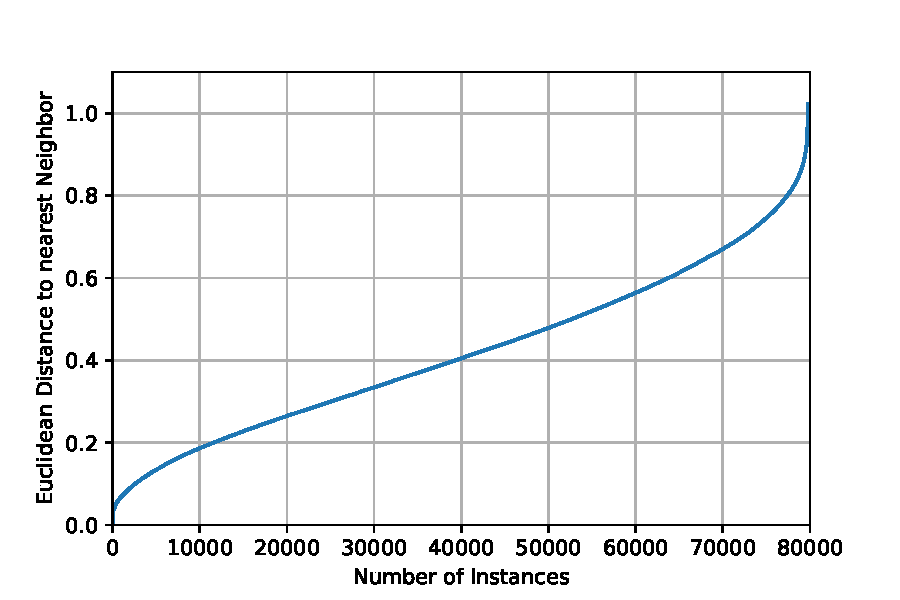
\includegraphics[height=8cm]{Bilder/models/kneighbors.pdf}
	\caption{Each Instance's Distance to the nearest neighboring Point}
	\label{fig:dbscan-plot}
\end{figure}

This can be done with the algorithm \lstinline|sklearn.neighbors.NearestNeighbors|, which takes the input of a dataset with arbitrary dimensions. Using a specified distance metric, the algorithm outputs the distance of each data point to its nearest neighbor in the data set. The distance metric used is the euclidean distance.
The distance search shows that almost all points are within a maximum distance of 0.8 to the next neighbor. All other points are outliers and will be filtered out with \ac{DBSCAN}.



\subsection{Preselect Documents with \ac{DBSCAN}}
The \ac{DBSCAN} algorithm outputs, apart from clusters, outlier data points which do not belong into any cluster. With this algorithm, outliers in the data are detected to prevent the main clustering algorithm (KMeans) from overfitting. 
The clustering algorithm has the parameters \lstinline|eps| and \lstinline|metric| which tune the model.

The (distance) \lstinline|metric| is of course cosine. The \lstinline|eps| stands for the maximal distance between two points to be considered a neighbor \cite{SklearnClusterDBSCAN}. As established before, the outliers are those points which are more than 0.4 units separated from the next data point. Therefore, \lstinline|eps| is set to 0.4. 

The \ac{DBSCAN} model identified the outlier data (\ref{fig:dbscan-outliers}), amounting to about 3\% of the data points. These data points are not included into clustering by k-Means.

\subsection{Determine the Number of Clusters}
The KMeans algorithm is parameterized with the number of clusters (\lstinline|n_clusters|). Since the algorithm itself is not able to determine the cluster count, this number has to be approximated.
Kodinariya an Makwana suggest several applicable methods, among them are rule of thumb, and the elbow method with a silhouette score \cite{kodinariyaReviewDeterminingCluster2013}.
A good point for starting with choosing $k$ is the rule of thumb $k \approx \sqrt{\frac{n}{2}}$ with n being the number of instances in the dataset. Other literature also names the approximation of $k \approx log(n)$, but \cite[p.~1749]{maierOptimalConstructionKnearest2009} showcase how $k$ should be chosen in the order of $n$. 

\begin{table}[!h]
	\centering
	\caption{Three possible estimates for the optimal $k$}
	\begin{tabular}{lll}
		\toprule
		\textbf{heuristic for best }$\mathbf{k}$                         & $\mathbf{k}$ &  \\
		\midrule
		$k \approx \sqrt{\frac{n}{2}}$ &  199 &  \\
		\midrule
		$k \approx log(n)$             & 12   &  \\
		\midrule
		$k \approx n$                  &  e.g. 10 000, 20 000& \\
		\bottomrule
		
	\end{tabular}

\label{table:heuristic-k}
\end{table}

With the elbow method, the silhouette score of clustering results for different values of $k$ are visualized. 

The silhouette score is a measure of how similar intra-cluster points are and at the same time how dissimilar inter-cluster points are. A silhouette score of 1, being the highest value, is the most desirable.

The silhouette score $s$ of each data point $i$ can be calculated with the following formula \cite[p.~94]{kodinariyaReviewDeterminingCluster2013}:
\[ s(i) = \frac{b(i) - a(i)}{\max\{a(i),b(i)\}} \]

The measure $a$ denotes the mean distance to other points in the same cluster as $i$. This is interpreted as the inter-cluster dissimilarity, the higher $a(i)$, the more $i$ doesn't belong into the cluster.

The measure $b$ stands for the mean distance between $i$ and the points in the nearest other cluster. To identify the nearest other cluster to the point $i$, all mean distances to points of each cluster are calculated. The cluster with the smallest mean distance between all its points and $i$ is the neighboring cluster. The measure $b$ is interpreted as the similarity of $i$ to other clusters.

Being calculated for every point, this measure always falls in the interval $[-1;1]$. For $S = 1$, the relationship of $a(i)$ and $b(i)$ has to be $a(i) \ll b(i)$ so that the denominator and divisor each tend to $b(i)$ resulting in $S = 1$. This would mean that the point $i$ would have to be very far away from points in other clusters and very near to its own cluster. The value $S = 1$ is therefore the most desirable.

For $S = 1$, the relationship of $a(i)$ and $b(i)$ has to be $a(i) \gg b(i)$ so that the denominator and divisor each tend to $-a(i)$ respective $a(i)$ resulting in $S = -1$. In distance terms this means that the point $i$ is very far away from its own cluster points and very close to points in the next nearest cluster.

Therefore, the task of the elbow method using the silhouette coefficient is to maximize $S$ while preventing overfitting.

The above mentioned estimates (Table \ref{table:heuristic-k}) are a starting point for choosing values for $k$ during the calculation of silhouette coefficients. The following simulation shows how the k-Means algorithm for these values of $k$ performed.

 \begin{figure}[!h]
	\centering
	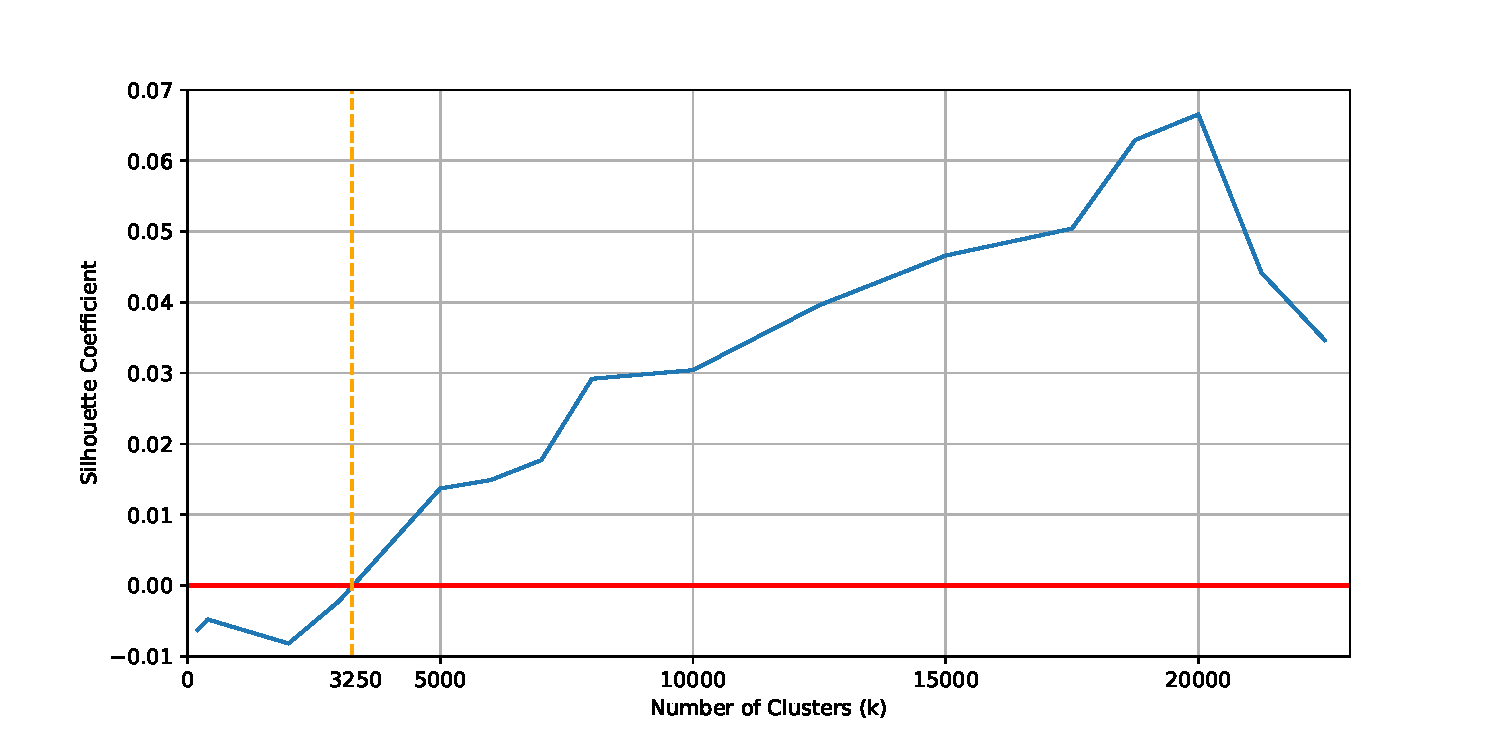
\includegraphics[width=0.95\textwidth]{Bilder/models/elbow.pdf}
	\caption{Each Instance's Distance to the nearest neighboring Point}
	\label{fig:silhouette}
\end{figure}

The chart \ref{fig:silhouette} shows how the silhouette coefficient behaves with respect to k-Means models with different numbers of clusters. The x-axis shows the number of clusters, which the algorithm was configured with. The diagram was created by executing several runs of \lstinline|MiniBatchKMeans|. In the used dataset, the DBSCAN algorithm already filtered out the outliers.

The chart shows how the silhouette coefficient falls under the 0 threshhold. A negative silhouette coefficient means that points in one cluster were misclassified as they are more close to other clusters. This is an indicator of underfitting. 

But not only the left hand side of the spectrum for $k$ can cause problems. When increasing $k$, the silhouette coefficient rises. In fact, one could obtain a perfect silhouette coefficient of 1 by assigning each point its own cluster \cite{yildirimTwoChallengesKMeans2020}. But with rising number of clusters, the generalization becomes lower. Again, the goal is a useful generalization. And dividing a group of 79741 documents into 20.000 groups can not be considered a useful generalization.

So, even though the silhouette method is very helpful as a technical analysis, the business goals have to be kept in mind. The silhouette coefficient at 0 means that on average, no points were misclassified due to underfitting. This minimal requirement is satisfied with $k$=3250.

\subsection{Train a KMeans Model}

The training with k=3250 takes about four minutes. Most clusters formed are in the size of 10 to 50 documents. The largest cluster contains 395 samples.

\begin{figure}[!h]
	\centering
	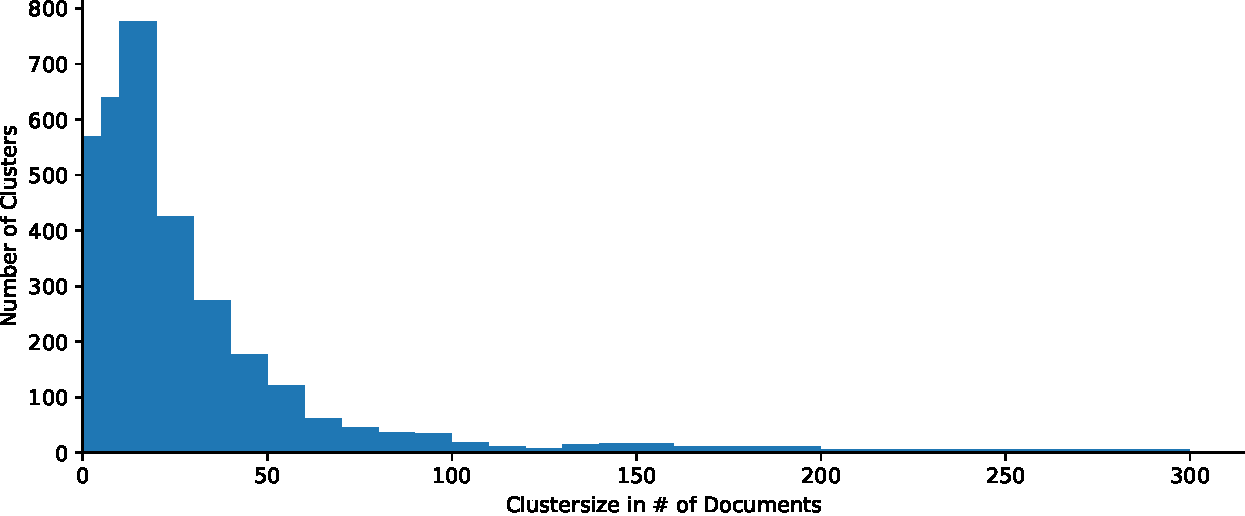
\includegraphics[height=6.5cm]{Bilder/models/clustersize.pdf}
	\caption{Distribution of the Cluster Sizes}
	\label{fig:clustersize}
\end{figure}

\subsection{Visualize Cluster Formation}
For visualizing, the \ac{t-SNE} algorithm is used. This projection allows to visualize the hundreds of dimensions of the embeddings in a two-dimensional representation. In Figure \ref{fig:kmeans}, the proximity of points stands for their close semantic relationship. Data points in the same color are contained in the same cluster. Since there are 3250 clusters, colors occur several times, even though they represent different clusters.

This Figure \ref{fig:kmeans} gives an overview on the clusters but doesn't show what is contained in the clusters. For this, each cluster needs a topic.

\begin{figure}[!ht]
	\centering
	\includegraphics[width=\linewidth]{Bilder/models/minibatchkmeans.pdf}
	\caption{All generated Clusters}
	\label{fig:kmeans}
\end{figure}


\newpage
\subsection{Generate Topics per Cluster}
\label{section:topics}
A topic consists of the three words with the highest document frequency in the cluster. A term-document-incidence matrix (see section \ref{section:tdim}) is a highly efficient method to find the top terms per cluster. This matrix is a binary matrix, representing whether a specific term is contained in a document. To find all terms in one cluster, first the documents (matrix rows) are selected. To find out the top terms, we simply calculate the column-wise sum. Since the data is binary, the sum denotes how many documents in the cluster contain this word. The maximum value is the number of documents in the cluster. The three words with the highest value are the topics of the cluster.

Each cluster has its own topic, but for reasons of comprehensibility this section presents only selected clusters and their topics.

\begin{figure}[!h]
	\centering
	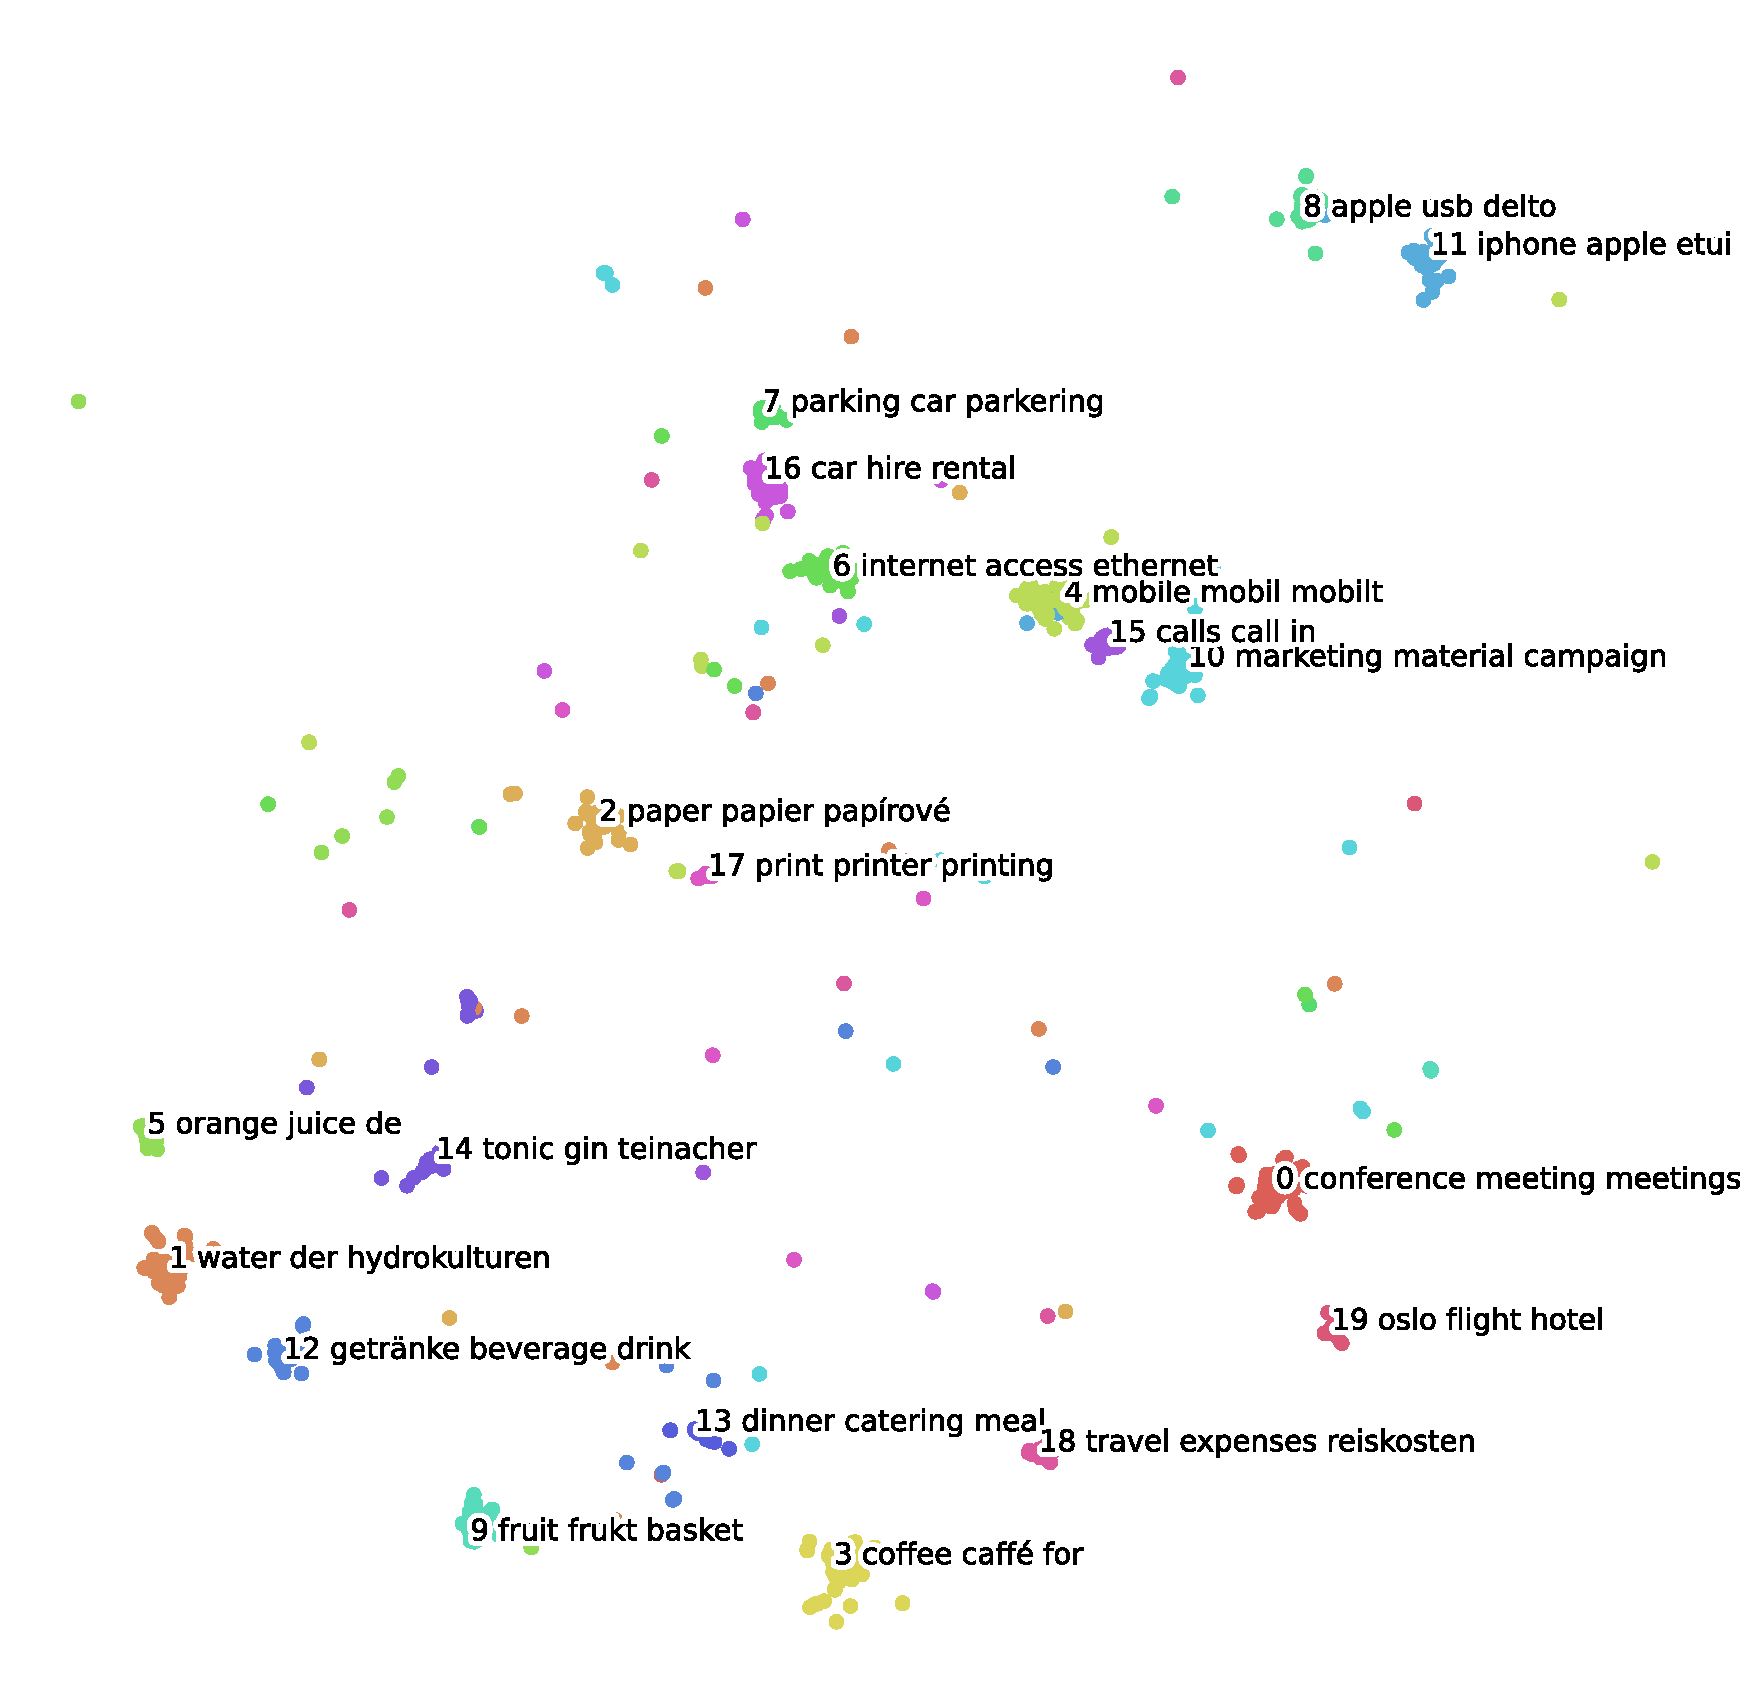
\includegraphics[width=\textwidth]{Bilder/models/topics.pdf}
	\caption{Selected Clusters and their Topics}
	\label{fig:topics}
\end{figure}

The chart \ref{fig:topics} seems to contain many outliers which are far away from their cluster. But, the outliers only appear to be so many, since the clusters are very dense. The chart contains more than 9000 data points, and most of them are so close to each other in one cluster, that they are indistinguishable from another.

What is striking about the clusters is the formation of areas where not only documents in one cluster are similar, but clusters are similar to each other. For example, clusters 5, 14, 1, and 12 form one area about drinking. Also, the four clusters are very close to 9 and 13. What too can be inferred is, that meals are connected with conferences through travel expenses. Additionally, these clusters are very far away from 8 and 11, which contain invoices on hardware. 

One proof, that the model captures the semantics of each word, is that the documents containing 'apple' (clusters 8, 11) are far away from the fruit basket cluster (cluster 9). The model understands, how in specific contexts 'Apple' stands for the brand and not the fruit.

Also in the north-western region of the chart, a cluster of clusters about services has formed. Although, a shorter distance between car renting (clusters 7, 16) and business travel (clusters 0, 18, 19) would be more understandable.

\include{Inhalt/04_Inhalt/content_evaluation}

\chapter{Deployment}
	The analysis results are targeted at decision-makers such as financial analysts and strategists. The clustering results can be part of a in-depth financial analysis, and provide a very broad overview on spending.
	
	The questions this overview should answer are:
	\begin{enumerate}
		\item Which spending categories exist?
		\item How does the spending divide onto the categories?
		\item Which magnitude exists between the different amounts spent?
		\item Which vendors are connected to the largest payments?
		\item Which geographical locations are related to the largest payments?
		\item How are the expenses distributed over all locations?
	\end{enumerate}
	
	The results of an analysis are often summarized using a business intelligence visualization tool. In this case, the analysis is visualized using Tableau.
	
	\begin{sidewaysfigure}
			\centering
		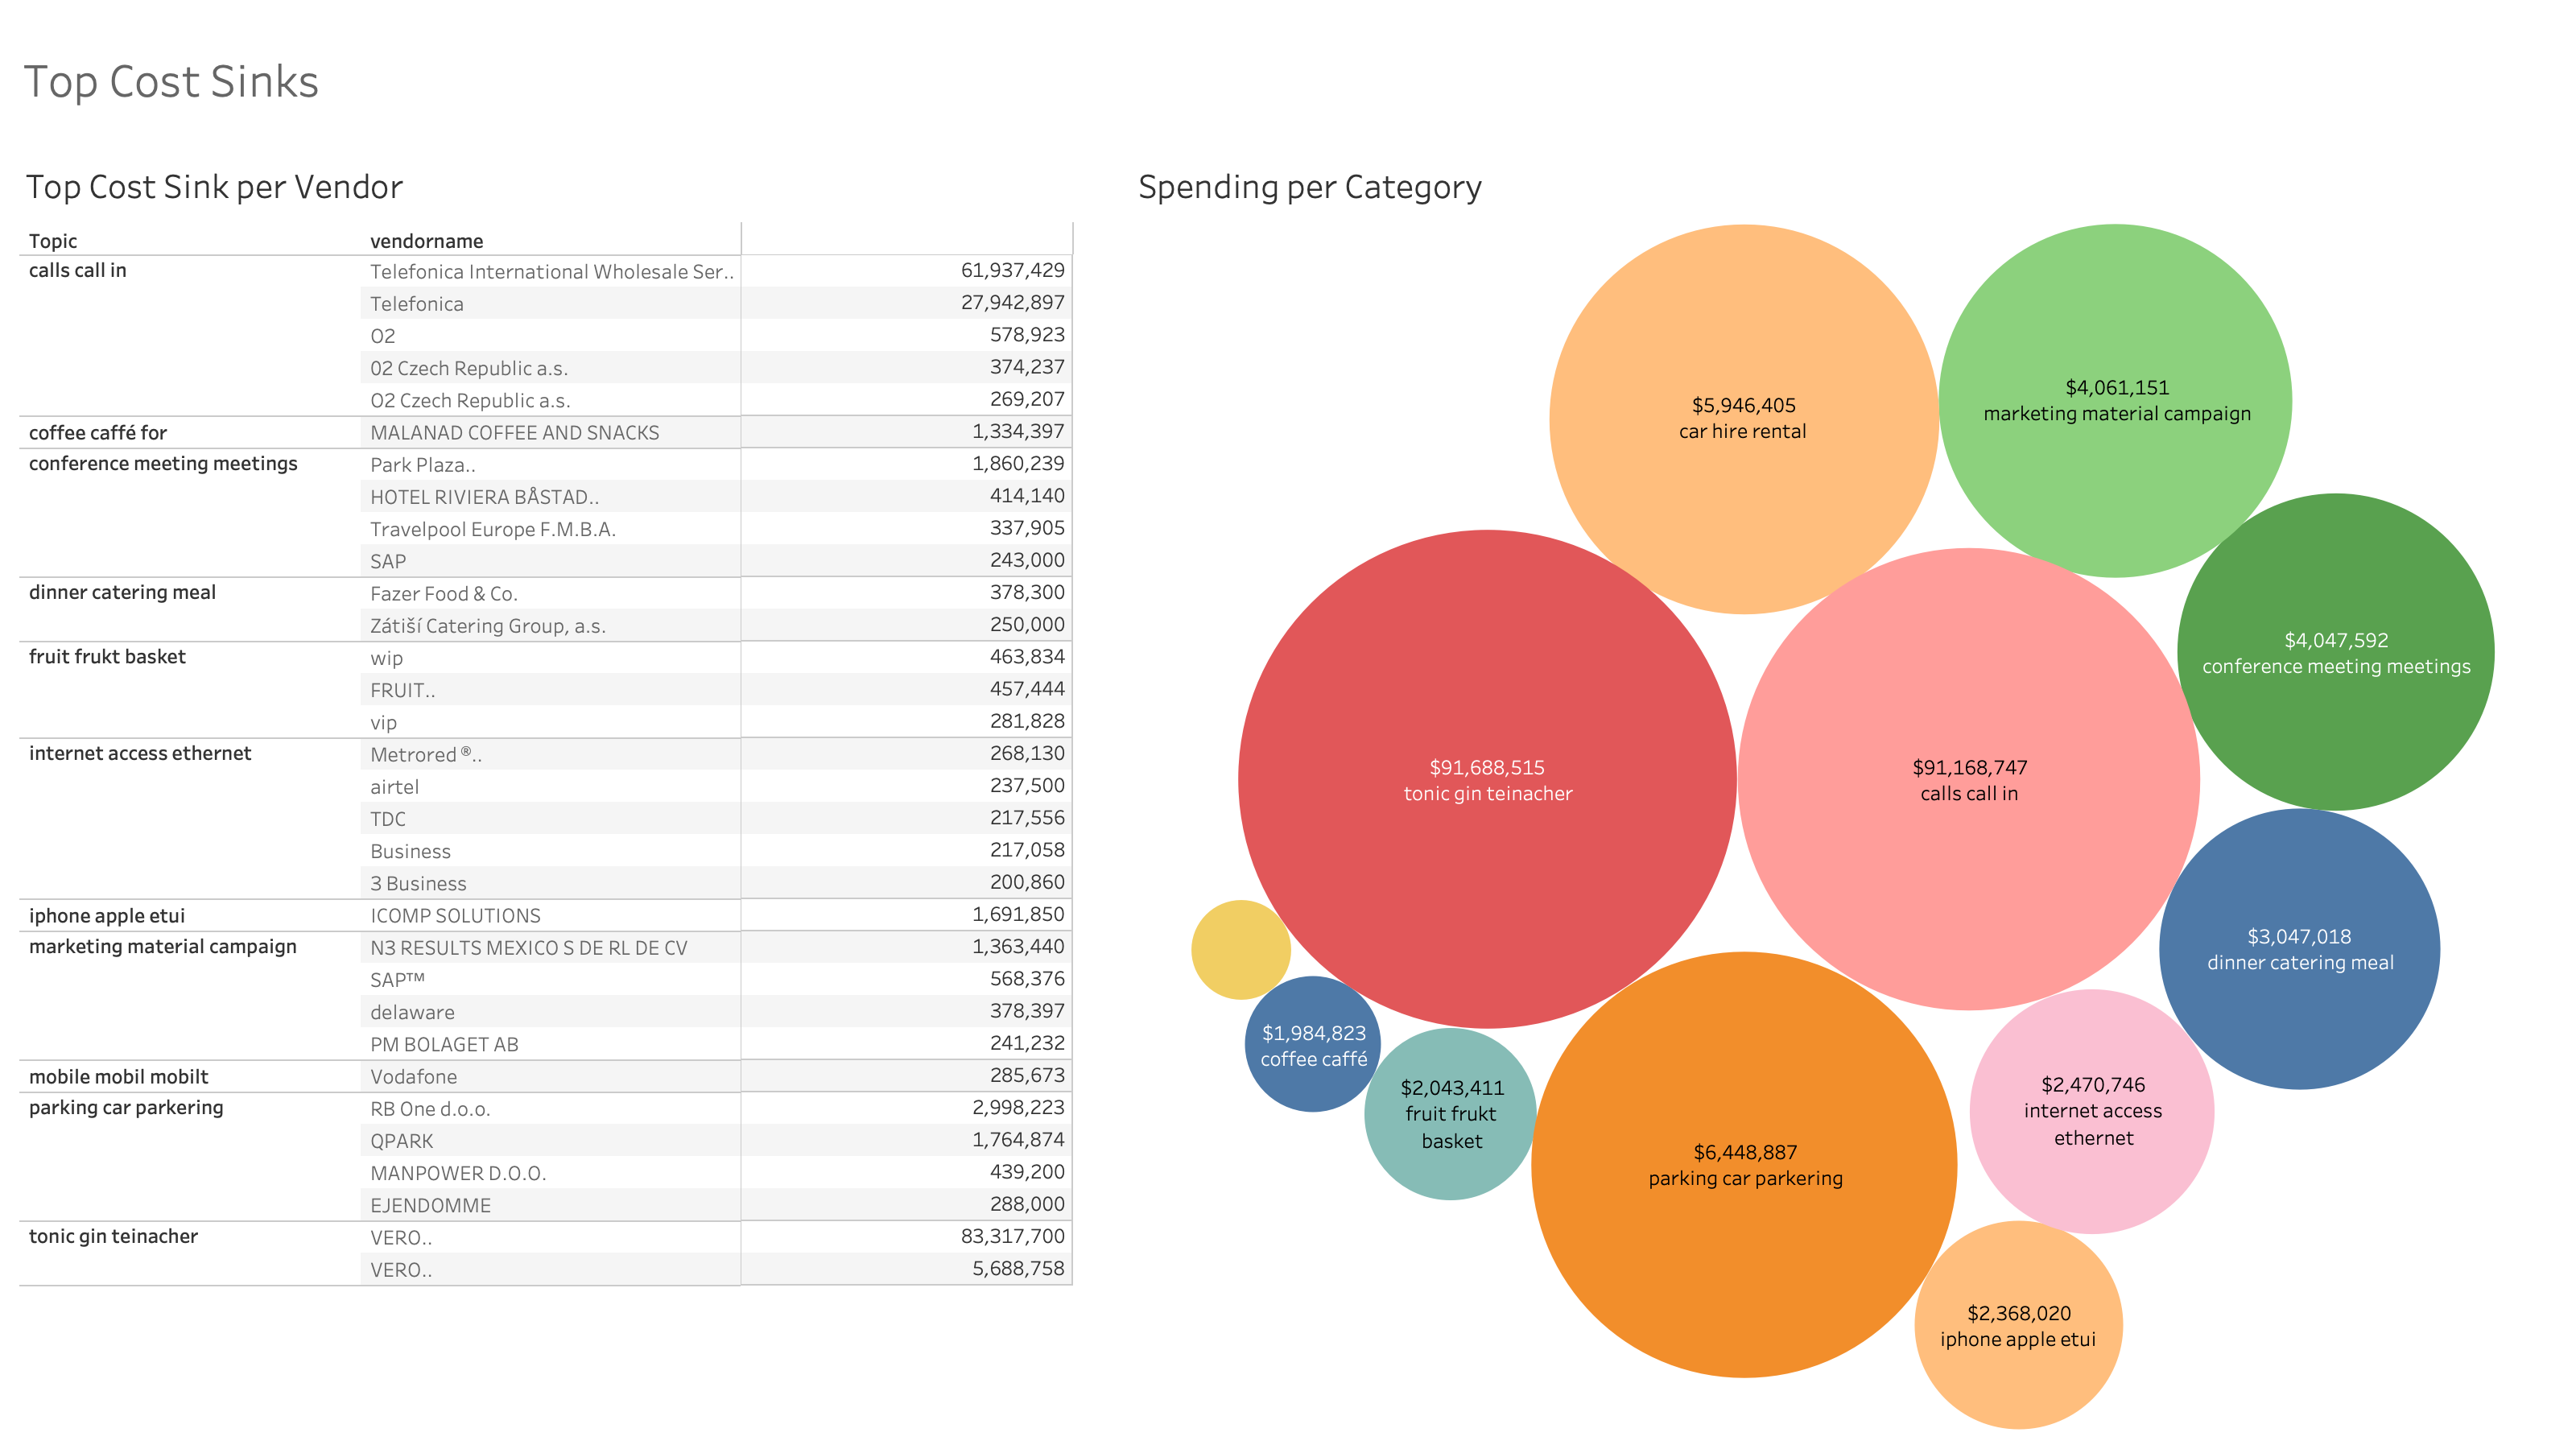
\includegraphics[
		width=\linewidth]{Bilder/deployment/bubble.png}
		\caption{Tableau Dashboard: Overview on the largest Spending Categories}
		\label{fig:dashboard-bubble}
	\end{sidewaysfigure}


\begin{sidewaysfigure}[h!]
	\centering
	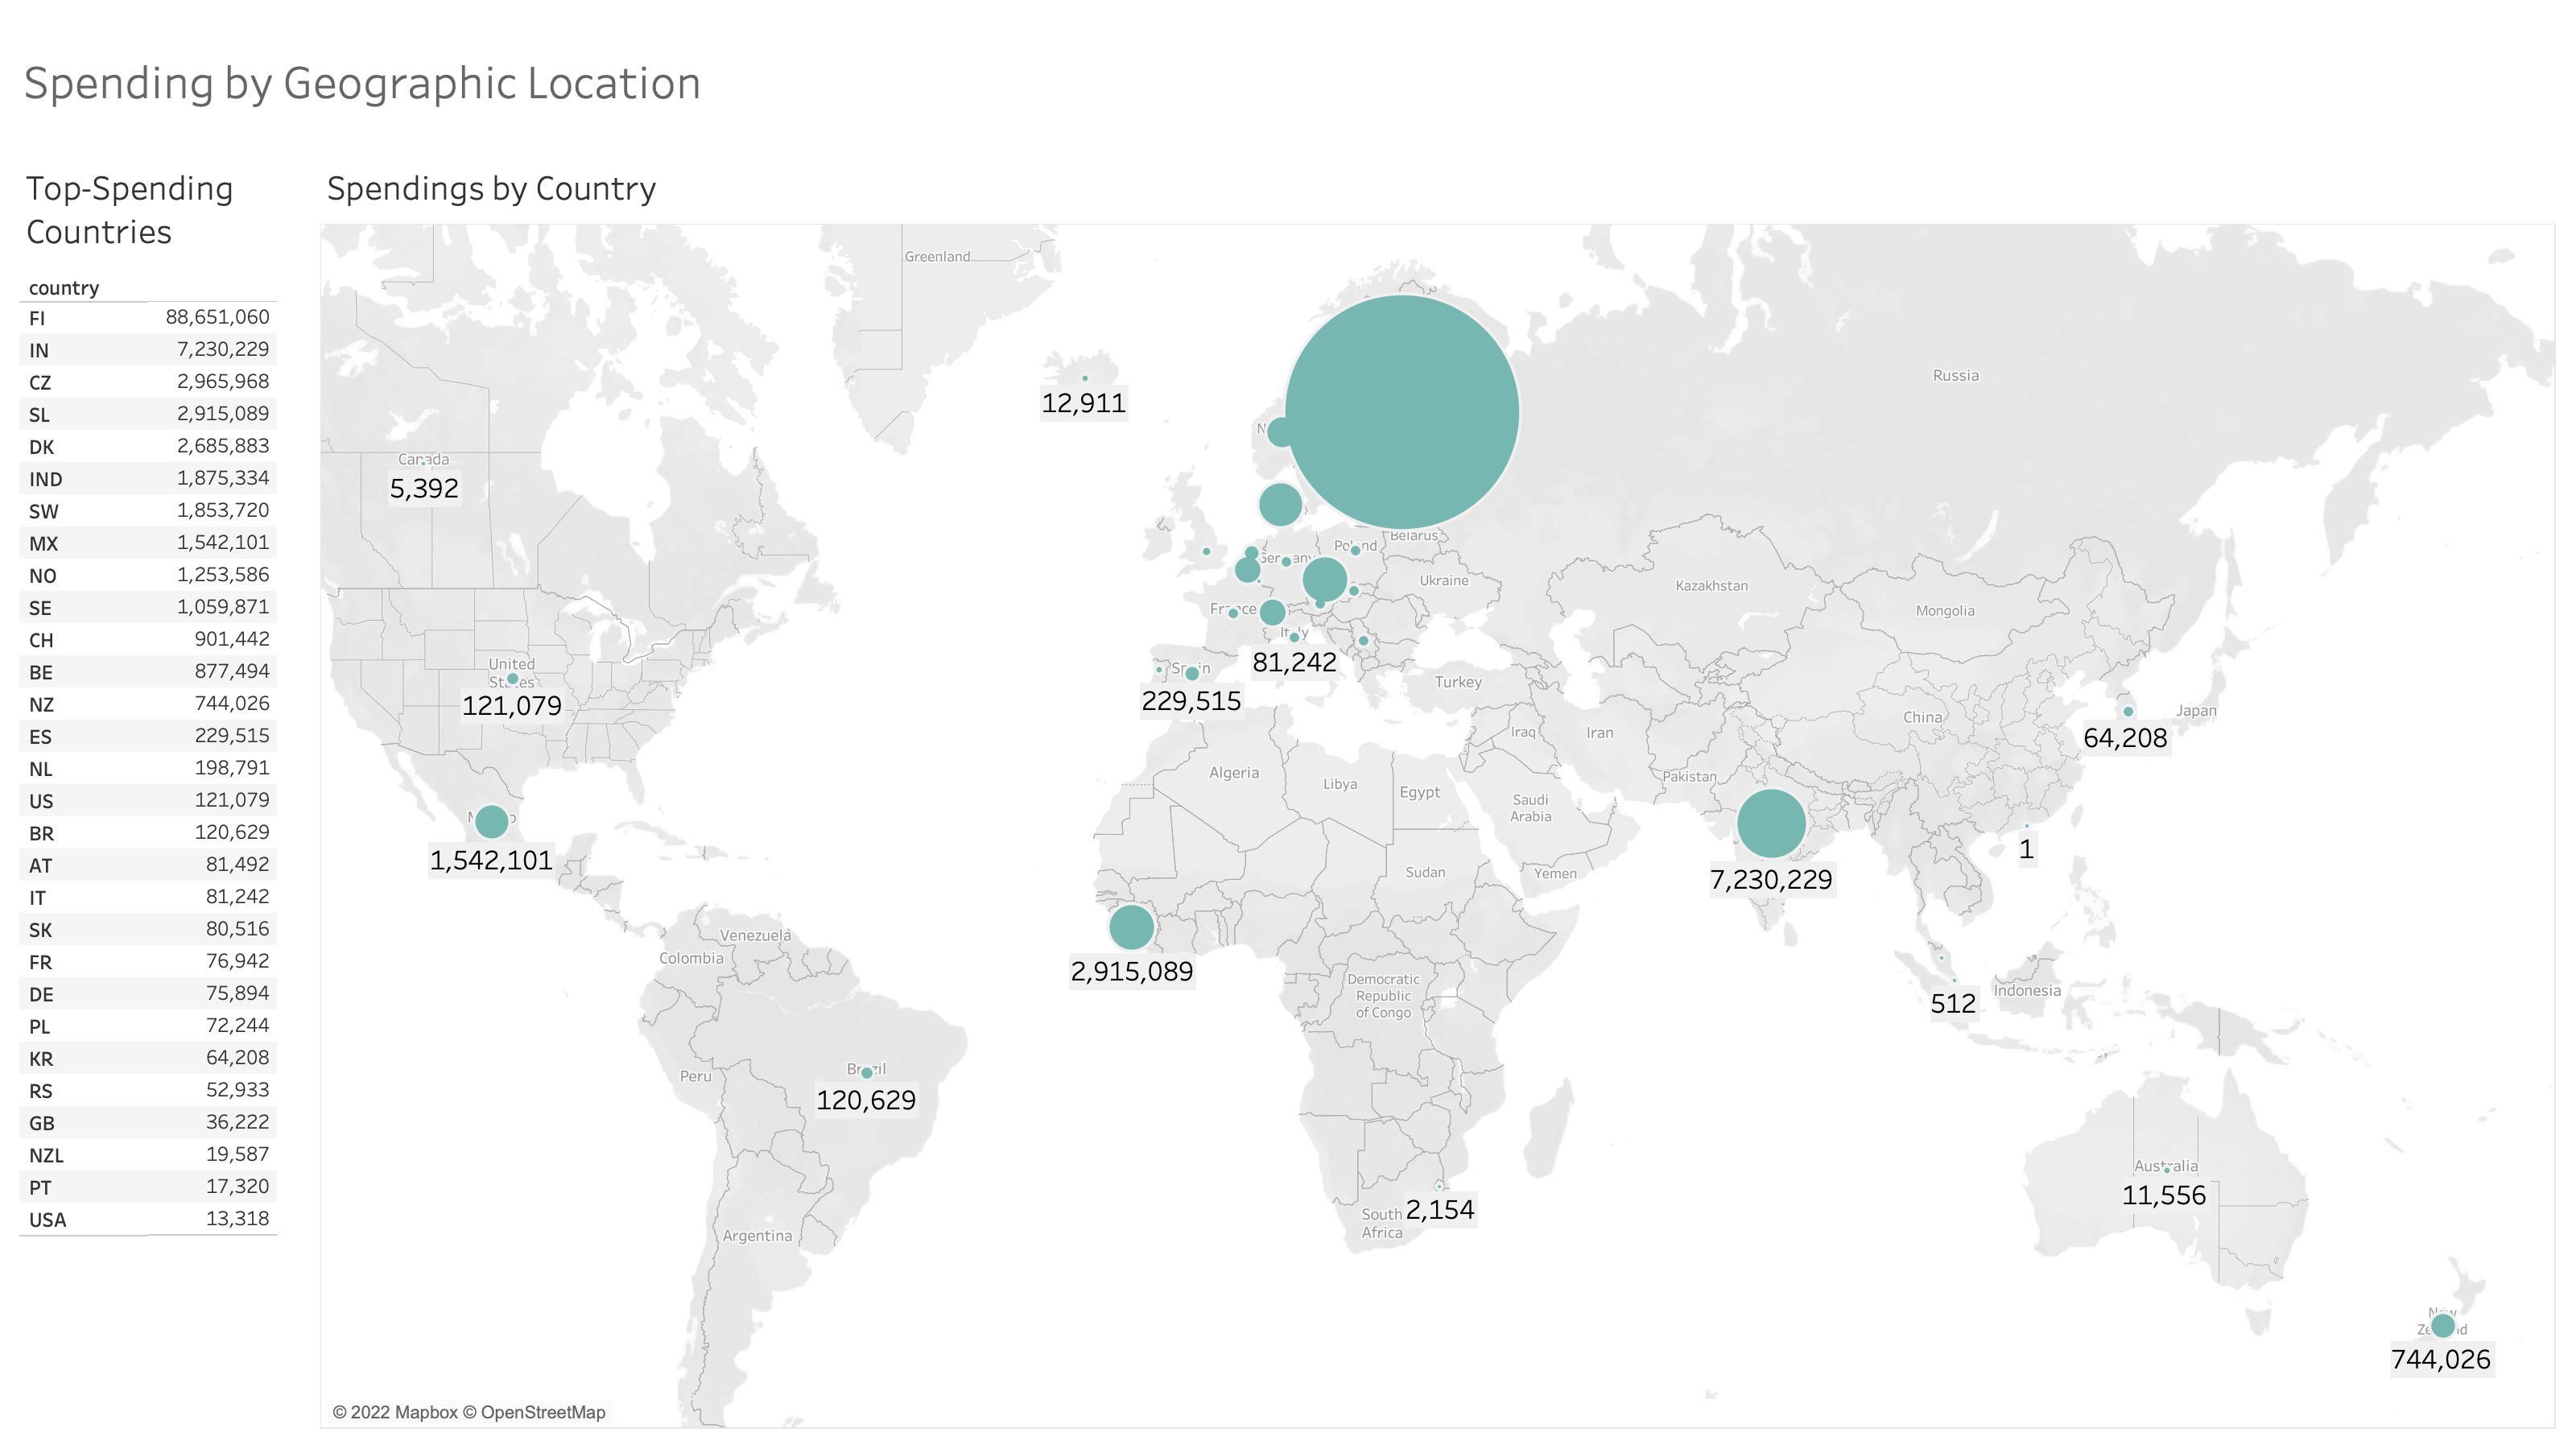
\includegraphics[width=\linewidth]{Bilder/deployment/world.png}
	\caption{Tableau Dashboard: Geographical Overview}
	\label{fig:dashboard-world}
\end{sidewaysfigure}

	The dashboard in Figure \ref{fig:dashboard-bubble} answers the questions 1-4. First, it shows the big picture of spending. Additional insights are in the tool tips of each bubble in the chart. The table on the left hand side provides a convenient overview of the different spending categories.
	
	The second dashboard in Figure \ref{fig:dashboard-world} concerns the questions 5 and 6. The map provides a quick insight into the impact of different company locations on spending. The information is shown with higher precision in the table on the left, which also gives a ranking of locations by expenses.


%\include{Inhalt/04_Inhalt/alternatives}
%\include{Inhalt/04_Inhalt/theoretical.tex}
%\include{Inhalt/04_Inhalt/practical.tex}

\chapter{Evaluation of the result}
Different Chapters in this thesis mention their respective objectives and criteria. This Chapter evaluated the result on the basis of these standards.

\paragraph{Detailed Task Description}
The goal of this thesis is adding value to real business documents by transforming unstructured data into a structured format. The structured information can then be used as a base for further analyses.
The task is to perform a full data analysis on the supplied dataset. The dataset is to be prepared for processing with established methods. An evaluation for different means of feature extraction, machine learning, model evaluation and visualization should be performed. With the evaluation a complete flow for the data processing should be presented. The result is an added value to the dataset by creating structured data and providing insights into this data.


\paragraph{Thesis Criteria}
Section \ref{section:criteria} mentions criteria for completing the task in the corporate environment. Firstly, only available resources should be used. All calculations were completed on the already available hardware. Also, all libraries used were open-source, needing no license. Tableau is free of charge for students. Finally, no internal services were required. This criterion is fulfilled.

Secondly, the dataset required special attention with respect to data protection. The data and the extraction results were only stored on SAP-authorized hardware. Additionally, the thesis contains a restriction notice to emphasize the special caution required.

Thirdly, the solution should be designed according to industry standards. The data mining follows industry standards by using state-of-the art models such as \ac{BERT}. Also, the Tableau dashboard presents the results in a way very common to this field. The research model used is the most popular and widely-used in the industry.

Fourth, the code needs proper documentation. The Jupyter Notebook format allows for combining Python code with markdown annotations. The resulting files are a great device for telling the story of the data analysis. The code is structured using headings to signify different logical units.

Fifth, the code should be optimized in its performance. A very careful choice of data structures based on benchmarks ensures the efficiency of the source code. Storage formats like the Python \lstinline|pickle| persist the information in a memory-saving way. Also, the used parallel processing speeds up processing times.

\paragraph{Business Objectives}
The business objectives (Section \ref{section:business-objectives}) firstly specify the goal of insight into spending across different related spending. The topics generated in Subsection \ref{section:topics} summarize detailed cost into cross-cutting topics such as beverages. 


%The primary goal is the development of a solution for automatic aggregation of documents, based on topics addressed in those documents. The focus is on shorter text segments, such as product descriptions. The business objective is an information gain, on how spending is distributed among cross-cutting topics in a company.
%The created solution can be evaluated with the business success criterion: "Does the solution identify and give useful insights in the money pits?". The judgment of goal achievement is a subjective matter. Evaluating the success should therefore be distributed among several stakeholders, including but not limited to the author, the supervisor and the supplier of the data.

Section \ref{section:business-objectives} also states the clear business success criterion: "Does the solution identify and give useful insights in the money pits?". This criterion is definitely fulfilled. The dashboard clearly shows which categories take up the most funds.


\paragraph{Data Mining Goals}
The data mining goals (Section \ref{section:data-mining-goals}) are four very distinct points:
\begin{enumerate}
	\item Identifying and applying appropriate methods for feature extracting tailored to this type of dataset.
	\item Identifying and applying appropriate methods for clustering documents in this type of dataset.
	\item Identifying and applying appropriate methods for topic modeling with this type of dataset.
	\item Aggregating expenses by their clusters and visualizing the output.
\end{enumerate}


%1. Identifying and applying appropriate methods for feature extracting tailored to this type of dataset.
Firstly, the feature extraction. The part about feature extraction (Section \ref{section:feature-extraction}) presents and carefully evaluates different methods with respect to their relevance to the specific dataset. The chosen mechanism \ac{BERT} is able to fulfill all requirements, while also reflecting the current state of the art. The resulting features provide best conditions for clustering documents.

%2. Identifying and applying appropriate methods for clustering documents in this type of dataset.
Secondly, the document clustering.
%How were the methods identified?
The clustering methods are evaluated on the basis of their ability to produce meaningful clusters. 
%Which methods were this?
Both k-Means and \ac{DBSCAN} are contrasted. 
%Which method was chosen?
The k-Means algorithm is able to generate higher-quality clusters in this special domain. While \ac{DBSCAN} technically produces more clear clusters, the proximity of documents such as used in k-Means is more meaningful than being connected to each other in a high-density area.
%How good were the results?
The clusters are created with the goal of a major generalization. Therefore, in the trade off between sharp clusters (high $k$) and strong ability to generalize (lower $k$), the lowest viable number of clusters is chosen. The high quality of the results is most obvious in the very intuitive arrangement of topics in a plane (Section \ref{fig:topics}).

%3. Identifying and applying appropriate methods for topic modeling with this type of dataset.
Thirdly, the topic modeling.
% Which method for topic modeling was chosen?
The topic model generates a topic which aims to describe all documents in one cluster. The model does so by choosing three word which are highly relevant to all contained documents. 

%4. Aggregating expenses by their clusters and visualizing the output.
Fourth, the visualization.
% how are the clusters visualized
A bubble chart (Figure \ref{fig:dashboard-bubble}) shows each cluster. The size of a bubble represents the magnitude of spending in this category.
% what does the visualization tell you?
The visualization gives an easily comprehensible representation of spending. 

\paragraph{Research Questions}
%How can information from invoice-like documents be extracted? 
The thesis answers both research questions. Firstly, it presents options to extract information from invoice-like documents. With means of annotation services, careful data wrangling and data cleaning, the data is transformed into a fitting format. A language model encodes the data for further processing.Then, the data is processed with means of unsupervised machine learning. A new information is gained: there are now groups of documents which are similar to each other.

%How can extracted information provide insights?
Secondly, the extraction results provide meaningful insights by uniting the information about a group of documents with the associated cost. One can now easily see how much is spent on each group.
\include{Inhalt/04_Inhalt/Outlook}
% ---- Literaturverzeichnis
\cleardoublepage
\renewcommand*{\chapterpagestyle}{plain}
\pagestyle{plain}
\pagenumbering{Roman}                   % Römische Seitenzahlen
\setcounter{page}{\numexpr\value{savepage}+1}
\printbibliography[title=References]

% ---- Anhang
\appendix
%\clearpage
%\pagenumbering{Roman}  % römische Seitenzahlen für Anhang
\chapter{Appendix}
\section{Inventory of Resources}

The inventory of resources is a list of all available utilities.
\begin{table}[!ht]
    \caption{Inventory of Resources}
    \begin{tabular}{lll}
    \toprule	
    \textbf{Type of resources} & \textbf{Kind of Resources} & \textbf{Quantification}                                                    \\
    \midrule
    Personnel                  & business experts           & 1 person                                                                   \\
								\cmidrule{2-3}
                               & data experts               & 1 person                                                                   \\
							   \cmidrule{2-3}
							   & technical support          & 1 person                                                                   \\
							   \cmidrule{2-3}	
							   & data mining experts        & 1 person                                                                   \\
    \midrule
    Data                       & fixed extracts             & -                                                                \\
								\cmidrule{2-3}
                               & live data                  & -                                                                          \\
							   \cmidrule{2-3}
                               & warehoused data            & -                                                                          \\
							   \cmidrule{2-3}
                               & operational data           & 1 dataset                                                                         \\
    \midrule
    Computing resources        & hardware platforms         & \begin{tabular}[c]{@{}l@{}}1 machine, access to \\  SAP AI Core\end{tabular} \\
    \midrule
    Software                   & data mining tools          & anaconda, jupyter                                                          \\
								\cmidrule{2-3}
                               & other relevant software    & Excel, Visual Studio Code, Git                                               \\
    \bottomrule                      
    \end{tabular}
    \label{tabelle:inventory}
    
    
  
    \end{table}


\cleardoublepage


\section{Invoice Header Data}
\begin{multicols}{2}
	\label{invoice-header}
	\begin{itemize}
		\setlength\multicolsep{0pt}
\item[] accountNumber.key
\item[] accountNumber.value
\item[] barCode.value
\item[] buyerAddress.cityTownVillage.value
\item[] buyerAddress.country.value
\item[] buyerAddress.district.value
\item[] buyerAddress.extraName.value
\item[] buyerAddress.full.key
\item[] buyerAddress.full.value
\item[] buyerAddress.houseNumber.value
\item[] buyerAddress.stateProvince.value
\item[] buyerAddress.street.value
\item[] buyerAddress.zip.value
\item[] buyerName.key
\item[] buyerName.value
\item[] comments.key
\item[] comments.value
\item[] country.value
\item[] currency.key
\item[] currency.value
\item[] deliveryDate.key
\item[] deliveryDate.value
\item[] deliveryNoteNo.key
\item[] deliveryNoteNo.value
\item[] discount.key
\item[] discount.value
\item[] dueDate.key
\item[] dueDate.value
\item[] employeeName.key
\item[] employeeName.value
\item[] exchRate.key
\item[] exchRate.value
\item[] exchRateSrcCurr.key
\item[] exchRateSrcCurr.value
\item[] exchRateTarCurr.key
\item[] exchRateTarCurr.value
\item[] filename
\item[] index
\item[] invoiceAmount.key
\item[] invoiceAmount.value
\item[] invoiceDate.key
\item[] invoiceDate.value
\item[] invoiceNo.key
\item[] invoiceNo.value
\item[] invoiceType.value
\item[] language
\item[] paymentTerms.key
\item[] paymentTerms.value
\item[] pii.address.key
\item[] pii.address.value
\item[] pii.email.key
\item[] pii.email.value
\item[] pii.name.key
\item[] pii.name.value
\item[] pii.other.key
\item[] pii.other.value
\item[] pii.phone.key
\item[] pii.phone.value
\item[] purchaseOrderNo.key
\item[] purchaseOrderNo.value
\item[] shipToAddress.cityTownVillage.value
\item[] shipToAddress.country.value
\item[] shipToAddress.district.value
\item[] shipToAddress.extraName.value
\item[] shipToAddress.full.key
\item[] shipToAddress.full.value
\item[] shipToAddress.houseNumber.value
\item[] shipToAddress.stateProvince.value
\item[] shipToAddress.street.value
\item[] shipToAddress.zip.value
\item[] shippingAmount.key
\item[] shippingAmount.value
\item[] subtotalAmount.key
\item[] subtotalAmount.value
\item[] tableHeader.batchNumber.value
\item[] tableHeader.description.value
\item[] tableHeader.discount.value
\item[] tableHeader.materialNumber.value
\item[] tableHeader.purchaseOrderNumber.value
\item[] tableHeader.quantity.value
\item[] tableHeader.serialNumber.value
\item[] tableHeader.tableHeaderBox
\item[] tableHeader.tax10Amount.value
\item[] tableHeader.tax10Rate.value
\item[] tableHeader.tax1Amount.value
\item[] tableHeader.tax1Rate.value
\item[] tableHeader.tax2Amount.value
\item[] tableHeader.tax2Rate.value
\item[] tableHeader.tax3Amount.value
\item[] tableHeader.tax3Rate.value
\item[] tableHeader.tax4Amount.value
\item[] tableHeader.tax4Rate.value
\item[] tableHeader.tax5Amount.value
\item[] tableHeader.tax5Rate.value
\item[] tableHeader.tax6Amount.value
\item[] tableHeader.tax6Rate.value
\item[] tableHeader.tax7Rate.value
\item[] tableHeader.totalAmount.value
\item[] tableHeader.unitOfMeasure.value
\item[] tableHeader.unitPrice.value
\item[] tax10Amount.key
\item[] tax10Amount.value
\item[] tax10Description.key
\item[] tax10Description.value
\item[] tax10Rate.key
\item[] tax10Rate.value
\item[] tax1Amount.key
\item[] tax1Amount.value
\item[] tax1Description.key
\item[] tax1Description.value
\item[] tax1Rate.key
\item[] tax1Rate.value
\item[] tax2Amount.key
\item[] tax2Amount.value
\item[] tax2Description.key
\item[] tax2Description.value
\item[] tax2Rate.key
\item[] tax2Rate.value
\item[] tax3Amount.key
\item[] tax3Amount.value
\item[] tax3Description.key
\item[] tax3Description.value
\item[] tax3Rate.key
\item[] tax3Rate.value
\item[] tax4Amount.key
\item[] tax4Amount.value
\item[] tax4Description.key
\item[] tax4Description.value
\item[] tax4Rate.key
\item[] tax4Rate.value
\item[] tax5Amount.key
\item[] tax5Amount.value
\item[] tax5Description.value
\item[] tax5Rate.key
\item[] tax5Rate.value
\item[] tax6Amount.key
\item[] tax6Amount.value
\item[] tax6Description.key
\item[] tax6Description.value
\item[] tax6Rate.key
\item[] tax6Rate.value
\item[] tax7Amount.key
\item[] tax7Amount.value
\item[] tax7Description.value
\item[] tax7Rate.key
\item[] tax7Rate.value
\item[] tax8Amount.key
\item[] tax8Amount.value
\item[] tax8Description.value
\item[] tax8Rate.key
\item[] tax8Rate.value
\item[] tax9Amount.key
\item[] tax9Amount.value
\item[] tax9Description.value
\item[] tax9Rate.key
\item[] tax9Rate.value
\item[] totalAmount.key
\item[] totalAmount.value
\item[] vendorAddress.cityTownVillage.value
\item[] vendorAddress.country.value
\item[] vendorAddress.district.value
\item[] vendorAddress.extraName.value
\item[] vendorAddress.full.key
\item[] vendorAddress.full.value
\item[] vendorAddress.houseNumber.value
\item[] vendorAddress.stateProvince.value
\item[] vendorAddress.street.value
\item[] vendorAddress.zip.value
\item[] vendorBankAccountNo.key
\item[] vendorBankAccountNo.value
\item[] vendorName.key
\item[] vendorName.value
\item[] vendorTaxID.key
\item[] vendorTaxID.value
\end{itemize}
\end{multicols}
\cleardoublepage



\section{Invoice Line Item Data}
\begin{multicols}{2}
	\label{invoice-lines}
	\begin{itemize}
		\setlength\multicolsep{0pt}
		\item[] lineItem.batchNumber.value
		\item[] lineItem.description.value
		\item[] lineItem.discount.value
		\item[] lineItem.lineItemBox
		\item[] lineItem.materialNumber.value
		\item[] lineItem.purchaseOrderNumber.value
		\item[] lineItem.quantity.value
		\item[] lineItem.serialNumber.value
		\item[] lineItem.tax10Amount.value
		\item[] lineItem.tax10Rate.value
		\item[] lineItem.tax1Amount.value
		\item[] lineItem.tax1Rate.value
		\item[] lineItem.tax2Amount.value
		\item[] lineItem.tax2Rate.value
		\item[] lineItem.tax3Amount.value
		\item[] lineItem.tax3Rate.value
		\item[] lineItem.tax4Amount.value
		\item[] lineItem.tax4Rate.value
		\item[] lineItem.tax5Amount.value
		\item[] lineItem.tax5Rate.value
		\item[] lineItem.tax6Amount.value
		\item[] lineItem.tax6Rate.value
		\item[] lineItem.tax7Amount.value
		\item[] lineItem.tax7Rate.value
		\item[] lineItem.tax8Amount.value
		\item[] lineItem.tax8Rate.value
		\item[] lineItem.tax9Amount.value
		\item[] lineItem.tax9Rate.value
		\item[] lineItem.totalAmount.value
		\item[] lineItem.unitOfMeasure.value
		\item[] lineItem.unitPrice.value
	\end{itemize}
\end{multicols}
\newpage
\section{Benchmarking Python Data Structures}
\label{benchmarkDF}

The following benchmark of different indexing method shows the performance disparity between \lstinline|dictionaries| (maps) and \lstinline|DataFrame|s. A \lstinline|DataFrame| is a tabular data structure in Python. While the \lstinline|DataFrame| takes a few microseconds, accessing the same data in a \lstinline|dictionary| is up to 300 times faster.

\begin{figure}[h!]
	%\left
	\includegraphics[height=15cm]{Bilder/appendix/dfvsdict.png}
\end{figure}
\begin{lstlisting}[caption={Benchmark of Indexing with Python Data Structures}]
\end{lstlisting}
The \lstinline|.loc| indexing is  130.24 times slower than dictionary access.\\
The \lstinline|.at|  indexing is  62.06 times slower than dictionary access.\\
The \lstinline|.iloc|  indexing is  310.28 times slower than dictionary access.\\
The \lstinline|.iat|  indexing is  213.44 times slower than dictionary access.

\newpage
\section{Data Wrangling Script}
The following script processes one \ac{JSON} invoice file. This particular script only extracts the header data from the invoice and returns it as a \lstinline|DataFrame|.

\lstinputlisting[
label=code:InvoiceReader,    % Label; genutzt für Referenzen auf dieses Code-Beispiel
caption=Python Script for extracting JSON Data into a DataFrame,
captionpos=b,               % Position, an der die Caption angezeigt wird t(op) oder b(ottom)
style=EigenerPythonStyle,   % Eigener Style der vor dem Dokument festgelegt wurde
firstline=0,                % Zeilennummer im Dokument welche als erste angezeigt wird
lastline=23                 % Letzte Zeile welche ins LaTeX Dokument übernommen wird
]{Quellcode/reader}

\newpage

\section{Feature Extraction with \acs{TF-IDF}}
\label{appendix:tfidf}

The following \lstinline|DataFrame| shows the \ac{TF-IDF} representation of the dataset. There being only zeroes visible does not mean, it is empty. This just again shows how sparse the \ac{TF-IDF} matrix is.


\begin{figure}[!h]
	\centering
	\includegraphics[width=\textwidth]{Bilder/preprocessing/tfidf.png}
	\label{fig:tfidf}
	\caption{Features extracted with TF-IDF}
\end{figure}

When selecting ten random documents, and summing their weights, the values for each token show up. For the ten random documents, the word 'beer' is of the highest importance according to \ac{TF-IDF}.
\begin{figure}[!h]
	\centering
	\includegraphics[height=6cm]{Bilder/preprocessing/tfidf_sparse.png}
	\label{fig:tfidf_sparse}
	\caption{Ten words from the Vocabulary and their summed Weight}
\end{figure}


\newpage
\section{Transformer Architecture}

\begin{figure}[h!]
	\label{fig:transformer}
	\centering
	\includegraphics[height=18cm]{Bilder/preprocessing/BERT/transformer_architecture.png}
	\caption[The Transfomer Architecture]{The Transfomer Architecture \cite{transformersAttention}}
\end{figure}




\newpage
\section{Outliers detected with \acs{DBSCAN}}
This projection shows which data points were classified as outliers (marked red) by \ac{DBSCAN}. At first, it might seem confusing that the outliers are centered in the projection. But, this dataset has undergone tremendous dimensionality reduction - from 512 dimensions to just two. This process can simply not capture all distances in all dimensions, especially for this magnitude of compression. Instead, the \ac{DBSCAN} algorithm can be trusted to inspect all dimensions for outliers.
\begin{figure}[h!]
	\centering
	\includegraphics[height=15cm]{Bilder/models/outliers.pdf}
	\caption{Projection of the Data with Outliers marked Red }
	\label{fig:dbscan-outliers}
\end{figure}
\newpage
\end{document}
